\documentclass[11pt]{article}

% Change "review" to "final" to generate the final (sometimes called camera-ready) version.
% Change to "preprint" to generate a non-anonymous version with page numbers.
\usepackage[review]{acl}

% Standard package includes
\usepackage{times}
\usepackage{latexsym}

% For proper rendering and hyphenation of words containing Latin characters (including in bib files)
\usepackage[T1]{fontenc}
% For Vietnamese characters
% \usepackage[T5]{fontenc}
% See https://www.latex-project.org/help/documentation/encguide.pdf for other character sets

% This assumes your files are encoded as UTF8
\usepackage[utf8]{inputenc}

% This is not strictly necessary, and may be commented out,
% but it will improve the layout of the manuscript,
% and will typically save some space.
\usepackage{microtype}

% This is also not strictly necessary, and may be commented out.
% However, it will improve the aesthetics of text in
% the typewriter font.
\usepackage{inconsolata}

%Including images in your LaTeX document requires adding
%additional package(s)
\usepackage{graphicx}
% Prefer figures stored in ./paper/figure/, but fall back to the project-level ./figures/
\graphicspath{{figure/}{../figures/}}

% Math in the method section and the preference-pair diagram (fig_dpo_pairs.tex)
\usepackage{amsmath}
\usepackage{amssymb}
\usepackage{booktabs}
\usepackage{multirow}
\usepackage[table,dvipsnames]{xcolor} % before tikz, which loads xcolor without these options
\usepackage{tikz}
\usetikzlibrary{arrows.meta}
\usepackage[normalem]{ulem} % \sout for struck-out table rows

% Names printed by \autoref
\def\sectionautorefname{Section}
\def\subsectionautorefname{Section}
\def\appendixautorefname{Appendix}
\def\subappendixautorefname{Appendix}

% If the title and author information does not fit in the area allocated, uncomment the following
%
%\setlength\titlebox{<dim>}
%
% and set <dim> to something 5cm or larger.

\title{Preferenece-Tuned Generation and Selection Strategies of Synthetic Student Answers for Automatic Answer Scoring}

% Author information can be set in various styles:
% For several authors from the same institution:
% \author{Author 1 \and ... \and Author n \\
%         Address line \\ ... \\ Address line}
% if the names do not fit well on one line use
%         Author 1 \\ {\bf Author 2} \\ ... \\ {\bf Author n} \\
% For authors from different institutions:
% \author{Author 1 \\ Address line \\  ... \\ Address line
%         \And  ... \And
%         Author n \\ Address line \\ ... \\ Address line}
% To start a separate ``row'' of authors use \AND, as in
% \author{Author 1 \\ Address line \\  ... \\ Address line
%         \AND
%         Author 2 \\ Address line \\ ... \\ Address line \And
%         Author 3 \\ Address line \\ ... \\ Address line}

\author{First Author \\
  Affiliation / Address line 1 \\
  Affiliation / Address line 2 \\
  Affiliation / Address line 3 \\
  \texttt{email@domain} \\\And
  Second Author \\
  Affiliation / Address line 1 \\
  Affiliation / Address line 2 \\
  Affiliation / Address line 3 \\
  \texttt{email@domain} \\}

%\author{
%  \textbf{First Author\textsuperscript{1}},
%  \textbf{Second Author\textsuperscript{1,2}},
%  \textbf{Third T. Author\textsuperscript{1}},
%  \textbf{Fourth Author\textsuperscript{1}},
%\\
%  \textbf{Fifth Author\textsuperscript{1,2}},
%  \textbf{Sixth Author\textsuperscript{1}},
%  \textbf{Seventh Author\textsuperscript{1}},
%  \textbf{Eighth Author \textsuperscript{1,2,3,4}},
%\\
%  \textbf{Ninth Author\textsuperscript{1}},
%  \textbf{Tenth Author\textsuperscript{1}},
%  \textbf{Eleventh E. Author\textsuperscript{1,2,3,4,5}},
%  \textbf{Twelfth Author\textsuperscript{1}},
%\\
%  \textbf{Thirteenth Author\textsuperscript{3}},
%  \textbf{Fourteenth F. Author\textsuperscript{2,4}},
%  \textbf{Fifteenth Author\textsuperscript{1}},
%  \textbf{Sixteenth Author\textsuperscript{1}},
%\\
%  \textbf{Seventeenth S. Author\textsuperscript{4,5}},
%  \textbf{Eighteenth Author\textsuperscript{3,4}},
%  \textbf{Nineteenth N. Author\textsuperscript{2,5}},
%  \textbf{Twentieth Author\textsuperscript{1}}
%\\
%\\
%  \textsuperscript{1}Affiliation 1,
%  \textsuperscript{2}Affiliation 2,
%  \textsuperscript{3}Affiliation 3,
%  \textsuperscript{4}Affiliation 4,
%  \textsuperscript{5}Affiliation 5
%\\
%  \small{
%    \textbf{Correspondence:} \href{mailto:email@domain}{email@domain}
%  }
%}

\begin{document}
\maketitle
\begin{abstract}
Cross-Question generalization has long been a core challenge in Automatic Short Answer Scoring (ASAS), where a trained model generalizes poorly to unseen questions. 
In this paper, we explore various strategies to improve cross-question generalization of ASAS models via synthetic data augmentation.
We compare few-shot prompting, supervised fine-tuning, and level-contrastive preference tuning. To better utilize the large amount of generated data, we select among the generated answers using the probabilities that a panel of encoder-based judges, assigns to the requested level.
On BEETLE and SciEntsBank, we find that answers generated by prompting are much less diverse than real student answers and reduce the performance of the model with the increasing amount of synthetic training data, while fine-tuned generators match real diversity and consistently improve the model's performance on unseen questions and domains, with preference-tuned generation yielding the largest gains.
We further explore various filtering strategies based on these judge probabilities and find that retaining a mixture of answers where judges assign the requested label with confidence and uncertainty yields the best performance and scales well with the amount of synthetic data.
\end{abstract}

\section*{Limitations}

\section{Introduction}

Automatic short answer scoring (ASAS) is a critical task in educational assessment, where a model is trained to score student responses to open-ended questions.
Traditional approaches have largely relied on supervised learning from annotated answers to the same questions encountered at evaluation time, using either engineered features or neural representations \citep{burrowsErasTrendsAutomatic2015,riordanInvestigatingNeuralArchitectures2017}. As a result of supervised training, performance of these models often drops once confronted with unseen questions and domains.
Cross-question generalization, where a scorer must evaluate responses to questions absent from its training data, therefore remains an open challenge.
New questions introduce new target concepts, reference answers, and scoring criteria, which limit the transfer of patterns learned from seen questions \citep{dzikovskaSemEval2013Task2013,funayamaReducingCostCrossPrompt2023}.
Reducing this dependence on questions seen during training is critical for the practical deployment of ASAS systems, as it allows for the evaluation of student responses to new questions without requiring additional human annotation that is often not feasible in practical institutional contexts.

A large body of previous work tackles this challenge either by prompting large language models (LLMs) to score student answers~\citep{changAutomaticShortAnswer2024,chamiehLLMsShortAnswer2024} directly or by adapting the model architecture to better generalize to unseen questions~\citep{wangInjectRubricsShort2019,liSemanticFeatureWiseTransformation2021,funayamaReducingCostCrossPrompt2023,wuMatchingExemplarNext2023,sun-etal-2026-rubric}. There is also growing interest in using LLMs to synthesize training data for ASAS, to improve performance on unseen questions or address label imbalance \citep{yeZeroGenEfficientZeroshot2022,bexteLunchFreeOvercoming2025}. However, these works also show that student answers generated purely from LLM-prompting are less authentic and not always helpful for downstream training. 

Much existing work on data synthesis with LLMs for natural language understanding (NLU) has focused on general tasks such as sentiment analysis, intent detection, natural language inference (NLI), and topic classification~\citep{kumarDataAugmentationUsing2020,liSyntheticDataGeneration2023,zouFuseGenPLMFusion2024,ceginRoSERoundrobinSynthetic2025,pecherBetterGeneratorsClassifiers2026}, 
where labels usually carry a \textbf{fixed}, \textbf{input-independent} meaning that is often signaled by superficial lexical or semantic cues in the input text~\citep{joulinBagTricksEfficient2017,gururanganAnnotationArtifactsNatural2018,kaushikLearningDifferenceThat2020}.
ASAS differs from these tasks in two respects.
First, a useful synthetic answer must reflect a specific level of \textbf{understanding of the scientific concepts} involved, including partial knowledge and typical misconceptions, while also imitating the \textbf{linguistic style} of real students, such as informal phrasing and incomplete explanations.
Second, each score level's meaning is \textbf{question-specific}: it depends on the context and scoring criteria for each question rather than on fixed label semantics.
Established augmentation techniques that perturb seed examples from the training data via paraphrasing, insertion, or swapping~\citep{ceginLLMsVsEstablished2025} are therefore impractical, since surface-level edits cannot turn an answer to a seen question into an answer to a new one.

The goal of this paper is therefore to address these challenges by comprehensively investigating whether and how LLMs can synthesize realistic student responses to unseen open-ended science questions for ASAS training.

The contributions of this paper are as follows:
\begin{itemize}
    \item We propose a pipeline that uses existing annotated training data to synthesize new training data for out-of-distribution test data, e.g., unseen questions and domains. Since the pipeline requires only labeled examples, it can be readily applied to other NLU classification tasks.
    \item For this purpose, we investigate various ways of synthesizing realistic student responses to science questions for ASAS training, comparing few-shot prompting with synthesizers trained via supervised fine-tuning (SFT) and direct preference optimization (DPO) on annotated responses to seen questions. It turns out that a synthesizer trained on annotated responses to seen questions can readily generate realistic and useful synthetic responses to unseen questions, particularly when trained via DPO.
    \item Moreover, we investigate various synthetic answer selection strategies that rank candidates by the probability a panel of judges assigns to each answer's intended score level. We find that a mixture of answers where judges assign the requested label with confidence and uncertainty is the most useful for ASAS model training.
\end{itemize}

\section{Related Work}

\subsection{Synthetic Training Data for NLU}

A few papers investigate the use of synthetic data for training ASAS models. For instance, studies use LLMs to generate responses for underrepresented score levels~\citep{fangUsingGPT4Augment2024} or for new questions without annotated responses~\citep{bexteLunchFreeOvercoming2025}, finding that synthetic student answers are less realistic and are not helpful for training ASAS models. However, these studies rely mostly on prompting off-the-shelf LLMs and do not utilize the large number of real student responses to seen questions.

Beyond ASAS, data synthesis has been widely studied for other NLU tasks~\citep{fengSurveyDataAugmentation2021,longLLMsDrivenSyntheticData2024}.
Early work fine-tuned synthesizers on labeled examples with the class label prepended to the input and then sampled new examples for each class~\citep{anabytavorNotHaveEnough2020,kumarDataAugmentationUsing2020}.
With larger LLMs, later studies explored data synthesis by prompting with label-descriptive instructions and trained small task models on the generated data without any annotated examples~\citep{schickGeneratingDatasetsPretrained2021,yeZeroGenEfficientZeroshot2022,mengGeneratingTrainingData2022}.
Since synthetic data tends to be noisy and repetitive, some studies improve diversity through attribute-conditioned prompts, personas, or decoding interventions~\citep{yuLargeLanguageModel2023,chungIncreasingDiversityMaintaining2023,geScalingSyntheticData2025}.

Filtering the best synthetic data is another research focus. Methods range from simple length and formatting heuristics~\citep{yeZeroGenEfficientZeroshot2022} to LLM-based acceptance judgments~\citep{anikinaRigorousEvaluationLLM2025}. However, \citet{pecherBetterGeneratorsClassifiers2026} show that the gain from LLM-based filtering can still saturate as more synthetic data is added. Other approaches select examples by generation probability~\citep{mengGeneratingTrainingData2022} or using a classifier trained on real data~\citep{anabytavorNotHaveEnough2020}. \citet{zouFuseGenPLMFusion2024} measure how much several small task models disagree on the probability of a sample's synthetic label, and argue that a useful synthetic dataset contains both samples the models agree on, which aid convergence, and ambiguous samples on which they disagree, which improve generalization. They then use this signal to reweight the training data. Manual label correction can make additional synthetic answers useful for scoring~\citep{bexteLunchFreeOvercoming2025}. We train a panel of judges on the real training data and use their probability of the requested label as a quality signal to select synthetic answers for training.
% We investigate how judges trained on real student answers can guide selection for unseen questions and domains as the amount of synthetic data increases.

\citet{liSyntheticDataGeneration2023} further show that synthetic data is less effective for more subjective tasks, such as sarcasm detection. In ASAS, the boundaries between partially correct and fully correct or incorrect answers are often vague, so a successful synthesizer must capture partial understanding. 


\subsection{Pedagogical Role Simulation with LLMs} 
Though studies on synthesizing student responses with LLMs for downstream ASAS training are scarce, there is a growing body of work on simulating students or tutors with LLMs, predominantly in the context of mathematics tutoring dialogues.

For tutor simulation, \citet{macinaMathDialDialogueTutoring2023} paired human teachers with LLMs prompted to exhibit common student errors to collect the MathDial tutoring dataset.
For student simulation, researchers have conditioned simulated students on personality traits~\citep{liuPersonalityawareStudentSimulation2025} or cognitive levels~\citep{wuEmbracingImperfectionSimulating2025}.
Beyond dialogues, LLMs have been prompted to answer exam questions as students of different ability levels to estimate item difficulty~\citep{benedettoUsingLLMsSimulate2024} or to simulate student revisions for training feedback generators~\citep{nairClosingLoopLearning2024}.

Reinforcement learning has proven effective for both simulation tasks.
For tutors, simulated students provide reward signals, either via DPO on preference pairs ranked by a student model's predicted response correctness~\citep{scarlatosTrainingLLMbasedTutors2025} or via online training through multi-turn interactions with simulated students~\citep{dinucu-jianuProblemSolvingTeachingProblemSolving2025}.
As for student simulation, prompting alone cannot yield realistic answers: teachers who tutored the MathDial students reported that they \textbf{lacked authenticity}, used \textbf{overly complex} language, and were at times logically inconsistent~\citep{martynovaCanLLMsEffectively2025}.
Training on real student data helps: preference optimization yields far more realistic simulated students in tutoring dialogues than prompting~\citep{scarlatosSimulatedStudentsTutoring2026}, and DPO aligns simulated responses with student abilities estimated by item response theory (IRT) models~\citep{scarlatosSMARTSimulatedStudents2025}.
However, it is unclear whether such simulated student answers can be used to train ASAS models.

\section{Method}
\label{sec:method}

\autoref{fig:pipeline} provides an overview of our method. Details of the pipeline are described in the following subsections.

\begin{figure*}[t]
    \centering
    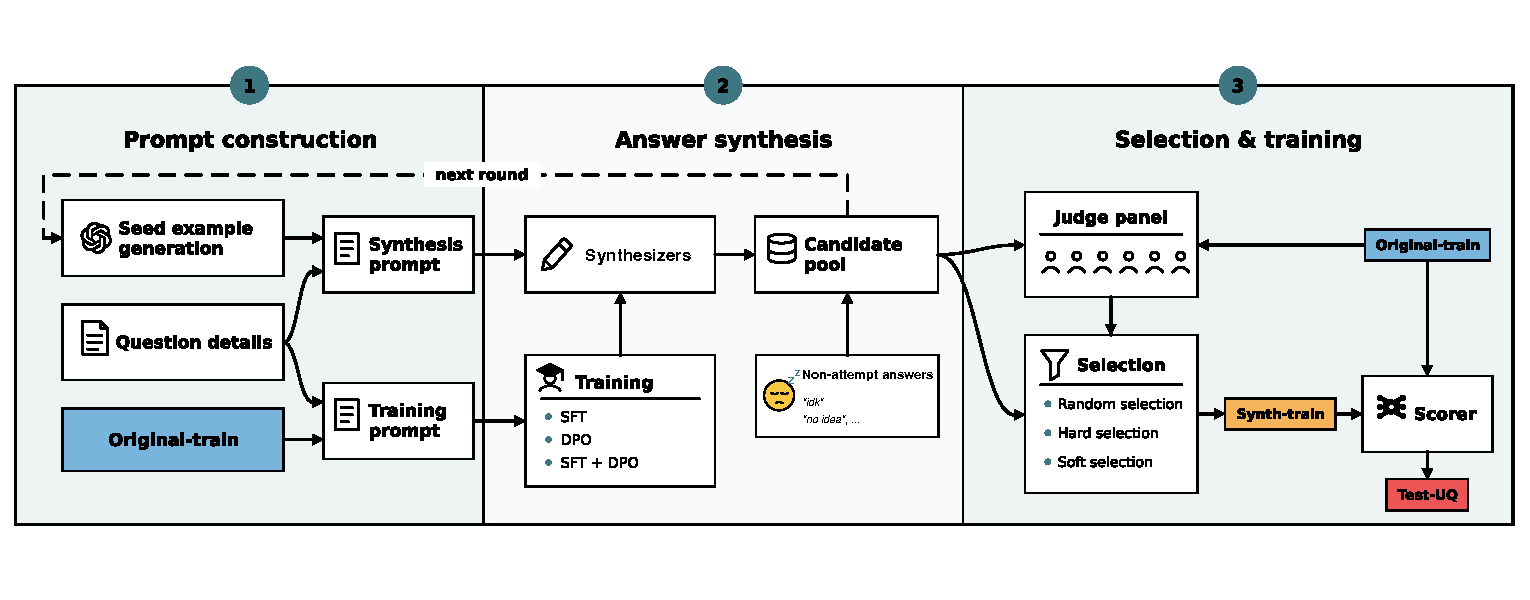
\includegraphics[width=\textwidth]{figures/fig1_pipeline.pdf}
    \caption{Overview of the training and evaluation pipeline.}
    \label{fig:pipeline}
\end{figure*}

\subsection{Dataset}
\label{sec:dataset}

% We use the three-way versions of BEETLE and SciEntsBank~\citep{dzikovskaSemEval2013Task2013}, with answers labeled incorrect, partially correct, or correct. Each example contains a question, a reference answer, a student answer, and its score level. \autoref{tab:dataset-statistics} summarizes the original training and test splits. UA denotes unseen answers, UQ denotes unseen questions, and UD denotes unseen domains. Our cross-question evaluation focuses on BEETLE UQ and SciEntsBank UQ and UD, whose questions are disjoint from the training questions; their real student answers are reserved for evaluation.

% For each split, we report the number of questions $Q$, the number of student answers $N$, and the mean number of answers per (question, score level) pair, $N/(3Q)$. This mean includes all three score levels for every question, including pairs with no observed answers. Training counts are reported before holding out 10\% of the original training set for validation.
We use the BEETLE and SciEntsBank datasets~\citep{dzikovskaSemEval2013Task2013}, reformulating the original five-way label scheme as a three-level scheme (incorrect, partially correct, correct), as in prior work~\citep{sun-etal-2026-rubric}. The unseen-question (UQ) and unseen-domain (UD) splits of SciEntsBank are used for cross-question evaluation. The latter one is a harder transfer task as it test the model on completely unseen subjects. \autoref{tab:dataset-statistics} in \autoref{app:datasets} summarizes the original training and test splits.

% \paragraph{Training Protocol}
% For the SFT synthesizers, we train for 800 steps. For the DPO synthesizers without SFT, we train for 1200 steps. For the DPO synthesizers with SFT, we train for 800 steps.

\subsection{Prompt Construction}
\label{sec:prompt-construction}

Each prompt is built for a question $q$ and a requested level $\ell$ and asks the model to generate new answers that differ from the seed examples. \autoref{tab:synthesis-prompt} in \autoref{app:synthesis-prompt} shows an example.

\paragraph{Question Context Augmentation.}
To better capture the requirements of each question and the scoring criteria for each level, \textit{gpt-5-mini} augments the question with a context description and a set of rubrics for each level. A detailed example of the question context and rubrics is shown in \autoref{tab:question-metadata} in \autoref{app:question-metadata}.

\paragraph{Seed Examples.}
During training, the seed examples are 10 real student answers from the training set for each question and level. For unseen questions, the seeds, contexts, and rubrics are derived from unlabeled answers pseudo-labeled by the judge panel (\autoref{app:seed-examples}).

\paragraph{Target Examples.}
To train the synthesizers via SFT or DPO, we randomly sample 10 real student answers from the training set for each question and level as the target examples.

\paragraph{Diversity Filter.}
To encourage diversity in the generated answers, we apply a diversity filter during training to the seed examples and the target examples, both \textbf{between} the targets and the seed examples and \textbf{among} the targets themselves. The cosine-similarity threshold between sentence embeddings\footnote{sentence-transformers/paraphrase-multilingual-mpnet-base-v2.} is 0.95, or 1.0 for correct answers, where \textbf{legitimate near-duplicates} are common.



\subsection{Answer Synthesis}
\label{sec:answer-synthesis}

We compare four synthesis approaches. Few-shot prompting uses off-the-shelf models, while the other three use models fine-tuned only on real answers to seen questions.

\paragraph{Few-shot prompting.}
As a baseline, synthesis prompts are sent directly to four instruction-tuned LLMs.\footnote{The full model list is given in \autoref{app:synthesizer-training}.}

\paragraph{Supervised fine-tuning (SFT).}
Each of the three open models is fine-tuned on the training prompts, with the real student answers as the target completions.



\paragraph{Level-contrastive preference tuning (DPO).}
Realistic synthetic answers for ASAS must capture the nuanced differences between adjacent score levels. SFT only raises the likelihood of the real answers at the requested level but never teaches the model to distinguish between adjacent levels, so we use direct preference optimization (DPO)~\citep{rafailovDirectPreferenceOptimization2023} on pairs of real answers (\autoref{fig:dpo-pairs}). For a training prompt $x$ with requested level $\ell$, the chosen completion $y^{+}$ lists real answers at level $\ell$, and the rejected completion $y^{-}$ lists real answers to the same question at an adjacent level $\ell'$, with $|\ell - \ell'| = 1$. The loss has two terms. The DPO term prefers $y^{+}$ over $y^{-}$, which teaches the synthesizer to separate adjacent levels. The NLL term is the SFT loss on $y^{+}$~\citep{pangIterativeReasoningPreference2024}: it maximizes the likelihood of the real answers at the requested level, since the DPO term alone only widens the margin and can lower the likelihood of $y^{+}$ itself.
\begin{gather}
\mathcal{L} = \mathbb{E}\Bigl[-\log \sigma\bigl(h_\theta(y^{+}) - h_\theta(y^{-})\bigr) + \alpha\,\mathcal{L}_{\mathrm{NLL}}(y^{+})\Bigr], \label{eq:dpo} \\
h_\theta(y) = \beta \log \frac{\pi_\theta(y \mid x)}{\pi_{\mathrm{ref}}(y \mid x)}. \notag
\end{gather}
Here $\pi_\theta$ is the synthesizer, $\pi_{\mathrm{ref}}$ is a frozen reference model, $\beta$ and $\alpha$ are hyperparameters (\autoref{app:synthesizer-training}), and $\mathcal{L}_{\mathrm{NLL}}$ is the per-token negative log-likelihood of $y^{+}$. Negative examples are filtered so that their answer lengths match those of the positive examples\footnote{We allow a difference of up to 10\% of the mean length.}, which prevents DPO from using 
\textit{length as a shortcut}, since answers tend to be longer at higher levels.

\begin{figure}[t]
    \centering
    \definecolor{dpochosen}{HTML}{2457A6}
    \definecolor{dporejected}{HTML}{B4472E}
    \begin{tikzpicture}[
        every node/.style={font=\scriptsize},
        prompt/.style={draw=black, fill=black!4, inner sep=3pt, outer sep=0pt, text width=0.96\columnwidth, align=left, anchor=north},
        level/.style={inner sep=3pt, text width=0.285\columnwidth, minimum height=1.95cm, align=flush center, anchor=north},
        chosen/.style={level, draw=black, thick, fill=dpochosen!10},
        rejected/.style={level, draw=black, dashed, fill=dporejected!6},
    ]
        \node[prompt, label={[anchor=south west, inner sep=1pt]north west:Prompt $x$}] (level) at (0,0) {\textbf{Requested level: partially correct}};
        \node[prompt] (x) at (level.south) {%
            \textbf{Question:} Explain why you got a voltage reading of 1.5 for terminal 1 and the positive terminal.\\
            \textbf{Context:} The question asks why a voltmeter read 1.5 V between terminal 1 and the positive terminal. \dots\\
            \textbf{Rubric:} States at least one of the necessary components correctly but omits others. \dots};
        \path (x.south) ++(0,-0.3) coordinate (row);
        \node[rejected] (incorrect) at ([xshift=-0.335\columnwidth]row) {\strut\textcolor{dporejected}{rejected $y^{-}$}\\[1pt]\textbf{Incorrect}\\[1pt]``because terminal one and the positive terminal are connected''\strut};
        \node[chosen] (partial) at (row) {\strut\textcolor{dpochosen}{chosen $y^{+}$}\\[1pt]\textbf{Partially correct}\\[1pt]``there was a gap''\\\mbox{}\\\mbox{}\\\mbox{}\strut};
        \node[rejected] (correct) at ([xshift=0.335\columnwidth]row) {\strut\textcolor{dporejected}{rejected $y^{-}$}\\[1pt]\textbf{Correct}\\[1pt]``because there is a gap between terminal one and the positive battery terminal''\strut};
        \draw[-{Latex[length=1.5mm]}, dashed, black] (incorrect.north |- x.south) -- (incorrect.north);
        \draw[-{Latex[length=1.5mm]}, very thick, black] (x.south) -- (partial.north);
        \draw[-{Latex[length=1.5mm]}, dashed, black] (correct.north |- x.south) -- (correct.north);
    \end{tikzpicture}
    \caption{Preference pairs for DPO. For a prompt that requests \textit{partially correct}, the chosen completion $y^{+}$ lists real answers at that level, and the rejected completion $y^{-}$ lists real answers at an adjacent level.}
    \label{fig:dpo-pairs}
\end{figure}


Two variants are trained. SFT+DPO continues from the SFT adapter, which also serves as $\pi_{\mathrm{ref}}$. DPO starts from the base model, which serves as $\pi_{\mathrm{ref}}$, and has no SFT stage.

\paragraph{Iterative generation.}
All models generate in rounds, shown by the dashed loop in \autoref{fig:pipeline}. In each round, every model receives one synthesis prompt per unseen question and requested level and returns 10 answers. The question-level ratio is kept balanced during generation. The synthetic answers join the seed examples for that question and level, so later prompts ask for answers that differ from earlier generations as well as from the initial seed examples. After the final round, we merge the answers of all models into one candidate pool.

\paragraph{Non-attempts.}
Real data also contain non-attempts such as ``idk''. These responses are largely question-independent and differ substantially from answers that attempt the question. To focus the synthesizers on substantive answers, non-attempts are excluded from synthesizer training and generated outside the main pipeline: a separate prompted LLM\footnote{GPT-4o-mini} writes a bank of non-attempts, all labeled incorrect. We also label each item in the training set if it is a non-attempt via an LLM, these answers are excluded from the sampling of seed and the target examples. 

\subsection{Selection and Training}
\label{sec:selection-training}

\paragraph{Judge panel and selection.}


Synthetic candidates vary in quality. \citet{zouFuseGenPLMFusion2024} use the probability given by an encoder-based judge as a quality signal to reweight the training instances. Following this idea, we score each candidate with a panel of $J = 6$ encoder-based judges trained only on the original training set (\autoref{app:judge-scorer}). For a candidate answer $a$ with requested level $\ell$, the panel score is the mean probability that the judges assign to $\ell$:
\begin{equation}
s(a) = \frac{1}{J} \sum_{j=1}^{J} p_j(\ell \mid a),
\label{eq:panel-score}
\end{equation}
where $p_j$ is the predictive distribution of judge $j$.
Various selection strategies are applied to the candidate pool. Detailed settings and results are given in \autoref{sec:results}.



\paragraph{Scorer.}
We combine the synthetic answers with the real training answers to train the scorer, an encoder-based classifier that predicts the score level. The models used for the judges and the scorers can be found in \autoref{app:judge-scorer}.

\section{Results and Analysis}
\label{sec:results}

% Generated by analysis_outputs/judge_uncertainty/build_random_arm_table.py
% Requires \usepackage{booktabs} and \usepackage[table,dvipsnames]{xcolor}.
\begin{table*}[t]
\centering
\small
\setlength{\tabcolsep}{3.6pt}
\begin{tabular}{lccccccccccccccc}
\toprule
 & \multicolumn{5}{c}{BEETLE UQ} & \multicolumn{5}{c}{SciEntsBank UQ} & \multicolumn{5}{c}{SciEntsBank UD} \\
\cmidrule(lr){2-6}\cmidrule(lr){7-11}\cmidrule(lr){12-16}
Synthetic amount & 1$\times$ & 2$\times$ & 3$\times$ & 4$\times$ & 5$\times$ & 1$\times$ & 2$\times$ & 3$\times$ & 4$\times$ & 5$\times$ & 1$\times$ & 2$\times$ & 3$\times$ & 4$\times$ & 5$\times$ \\
\midrule
w/o synthetic data & \multicolumn{5}{c}{61.2} & \multicolumn{5}{c}{56.5} & \multicolumn{5}{c}{53.8} \\
\midrule
Prompting & $-$0.3 & \cellcolor{BrickRed!18}$-$3.2 & \cellcolor{BrickRed!26}$-$4.5 & \cellcolor{BrickRed!35}$-$6.3 & \cellcolor{BrickRed!36}$-$6.4 & \cellcolor{BrickRed!16}$-$2.8 & \cellcolor{BrickRed!15}$-$2.7 & \cellcolor{BrickRed!18}$-$3.1 & \cellcolor{BrickRed!17}$-$3.0 & \cellcolor{BrickRed!24}$-$4.3 & \cellcolor{BrickRed!18}$-$3.2 & \cellcolor{BrickRed!25}$-$4.5 & \cellcolor{BrickRed!24}$-$4.3 & \cellcolor{BrickRed!25}$-$4.4 & \cellcolor{BrickRed!30}$-$5.4 \\
SFT & \cellcolor{Cerulean!5}+0.9 & \cellcolor{Cerulean!5}+0.9 & \cellcolor{Cerulean!11}+2.0 & \cellcolor{Cerulean!6}+1.1 & \cellcolor{Cerulean!8}+1.4 & \cellcolor{Cerulean!3}+0.5 & \cellcolor{Cerulean!6}+1.1 & \cellcolor{Cerulean!17}+3.0 & \cellcolor{Cerulean!13}+2.4 & \cellcolor{Cerulean!10}+1.9 & \cellcolor{Cerulean!18}+3.1 & \cellcolor{Cerulean!25}+4.4 & \cellcolor{Cerulean!24}+4.3 & \cellcolor{Cerulean!23}+4.0 & \cellcolor{Cerulean!24}+4.3 \\
SFT+DPO & +0.4 & \cellcolor{Cerulean!4}+0.8 & \cellcolor{Cerulean!8}+1.4 & \cellcolor{Cerulean!7}+1.2 & \cellcolor{Cerulean!11}+1.9 & \cellcolor{Cerulean!7}+1.3 & \cellcolor{Cerulean!9}+1.5 & \cellcolor{Cerulean!21}+3.7 & \cellcolor{Cerulean!14}+2.5 & \cellcolor{Cerulean!18}+3.1 & \cellcolor{Cerulean!23}+4.1 & \cellcolor{Cerulean!33}+5.8 & \cellcolor{Cerulean!36}+6.4 & \cellcolor{Cerulean!33}+5.9 & \cellcolor{Cerulean!35}+6.2 \\
DPO & \cellcolor{Cerulean!16}\textbf{+2.8} & \cellcolor{Cerulean!15}\textbf{+2.8} & \cellcolor{Cerulean!17}\textbf{+3.0} & \cellcolor{Cerulean!17}\textbf{+3.1} & \cellcolor{Cerulean!18}\textbf{+3.2} & \cellcolor{Cerulean!35}\textbf{+6.1} & \cellcolor{Cerulean!35}\textbf{+6.2} & \cellcolor{Cerulean!44}\textbf{+7.8} & \cellcolor{Cerulean!45}\textbf{+8.0} & \cellcolor{Cerulean!45}\textbf{+8.0} & \cellcolor{Cerulean!33}\textbf{+5.8} & \cellcolor{Cerulean!36}\textbf{+6.4} & \cellcolor{Cerulean!41}\textbf{+7.2} & \cellcolor{Cerulean!41}\textbf{+7.3} & \cellcolor{Cerulean!39}\textbf{+7.0} \\
\bottomrule
\end{tabular}
\caption{Differences between the performance of the ASAS model with and without synthetic data. \textbf{Bold} marks the best results per column. Each cell is an average of five random draws and four encoders.}
\label{tab:random-arm}
\end{table*}

\subsection{Diversity and Realism of Synthetic Answers}
\label{sec:realism-diversity}
% \noindent\textbf{Are the synthetic answers realistic and diverse enough?}

\vspace{0.5ex}
\noindent\colorbox{gray!15}{\parbox{\dimexpr\linewidth-2\fboxsep\relax}{%
Simple few-shot prompting with LLMs produces less diverse and less realistic answers than fine-tuned synthesizers.}}


\begin{figure}[t]
    \centering
    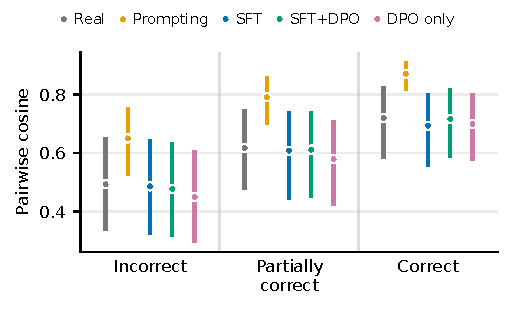
\includegraphics[width=0.8\columnwidth]{fig2_level_similarity_compact.pdf}
    \caption{Pairwise cosine similarity of answers within each correctness level, for real and synthetic answers.}
    \label{fig:level_similarity}
\end{figure}

\begin{figure}[t]
    \centering
    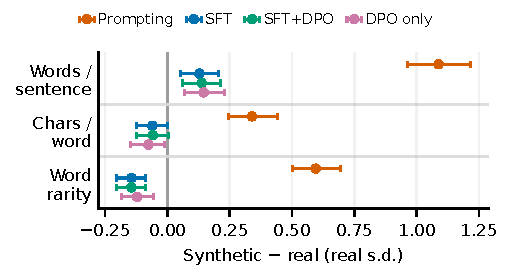
\includegraphics[width=0.8\columnwidth]{semantic_answer_style_metrics_compact.pdf}
    \caption{Difference in answer style metrics between synthetic and real answers. Word rarity is the mean word surprisal, $-\log_{10}$ of the add-half-smoothed word frequency in the benchmark's real training answers; out-of-vocabulary words, including misspellings, receive the maximum value.}
    \label{fig:style_metrics}
\end{figure}
Before using the synthetic answers for training, we first evaluate how \textbf{diverse} and \textbf{realistic} they are, which are crucial for effective data augmentation \citep{kumarDataAugmentationUsing2020,ceginChatGPTReplaceCrowdsourcing2023}. 

\noindent\textbf{Diversity} We measure semantic diversity as the pairwise cosine similarity of sentence embeddings among answers of the same correctness level, and compare it against that of the real answers~(\autoref{fig:level_similarity}). In principle, diversity naturally increases as the correctness level decreases because correct answers tend to be more homogeneous. The answers from the fine-tuned methods closely match the real answers in pairwise similarity across all levels, whereas the prompting method produces answers that are less diverse and more similar to each other.

\noindent\textbf{Realism} We measure realism as how closely the style of the synthetic answers matches that of the real student answers~(\autoref{fig:style_metrics}). For this, we compute the number of words in sentences, the mean number of characters per word, and the mean word rarity. Simply prompting the LLMs produces overly verbose and complex answers that deviate from the style of real student answers, while the fine-tuned synthesizers produce far more realistic answers. However, there is no significant difference among the three fine-tuned methods.

\subsection{Scoring Unseen Questions with Synthetic Answers}
\label{sec:scoring-unseen}

\vspace{0.5ex}
\noindent\colorbox{gray!15}{\parbox{\dimexpr\linewidth-2\fboxsep\relax}{%
Diverse and realistic synthetic student answers improve the performance of ASAS models on unseen questions, with the DPO approach achieving the best results. The positive and negative effects of each synthesizer persist as the amount of synthetic data increases.}}

We then train the ASAS model on the synthetic answers together with the original training data and evaluate it on the unseen questions. The synthetic answers are balanced across questions and levels and randomly sampled five times. By default, they match the size of the original training data, and we increase the amount up to five times this size. \autoref{tab:random-arm} reports the change in macro F1 relative to training on the original data only, and per-model scores are given in \autoref{tab:appendix-random-amount} (\autoref{app:per-model-results}).

At the default amount, prompting does not help and even lowers the macro F1 on SciEntsBank by around 3 points, consistent with its less realistic and less diverse answers (\autoref{sec:realism-diversity}). The three fine-tuned synthesizers improve the macro F1 in all settings, with SFT+DPO slightly ahead of SFT on SciEntsBank. DPO is the best in all three settings, improving the macro F1 by up to 6.1 points on SciEntsBank UQ.

Increasing the amount of synthetic data amplifies these effects. For the fine-tuned synthesizers the gains grow further, with most of the improvement reached at two to three times the original data size, while for prompting the loss keeps growing and reaches 6.4 points on BEETLE UQ at five times the size. This indicates that more realistic synthetic answers translate to better downstream performance, whereas unrealistic ones become more harmful the more of them are added.

Although the three fine-tuned synthesizers produce answers of similar style and diversity~(\autoref{sec:realism-diversity}), DPO method outperforms the others. We attribute the gap to level fidelity: the judge panel, trained only on real answers, assigns DPO answers to their requested level more often than answers from any other synthesizer~(\autoref{tab:judge-f1-by-arm} in~\autoref{app:judge-scorer}). This is consistent with the level-contrastive objective, which explicitly separates adjacent levels, whereas SFT only imitates answers at the requested level. 



\subsection{Judge-Based Selection}

\vspace{0.5ex}
\noindent\colorbox{gray!15}{\parbox{\dimexpr\linewidth-2\fboxsep\relax}{%
Selecting synthetic answers by judge probabilities filters out low-quality answers, and its benefit over random selection grows with the amount of synthetic data.}}


\begin{figure}[t]
    \centering
    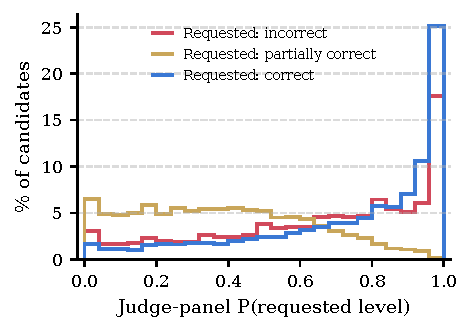
\includegraphics[width=0.8\columnwidth]{fig5_judge_probability.pdf}
    \caption{Distribution of the judge-panel probability $s(a)$ of the requested level, by requested level.}
    \label{fig:judge-probability}
\end{figure}

\begin{figure}[t]
    \centering
    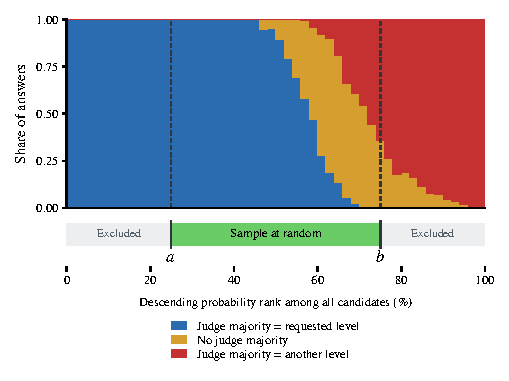
\includegraphics[width=0.8\columnwidth]{judge_hard_vote_group_share.pdf}
    \caption{Share of candidate answers by judge majority outcome, ranked by the panel probability assigned to the requested level.}
    \label{fig:judge-vote-share}
\end{figure}

\begin{figure}[t]
    \centering
    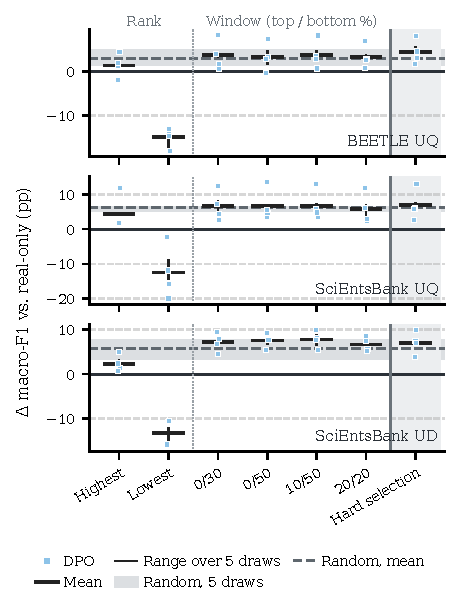
\includegraphics[width=0.8\columnwidth]{fig7_policy_summary_draws.pdf}
    \caption{Change in macro F1 relative to training on real data only for judge-based selection policies and random selection. Points show means and bars show ranges over five draws.}
    \label{fig:selection-policies}
\end{figure}

\begin{figure}[t]
    \centering
    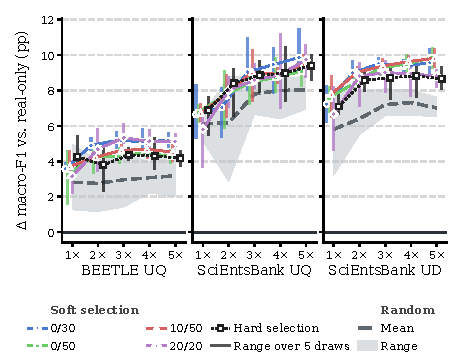
\includegraphics[width=0.8\columnwidth]{fig10_fraction_absolute.pdf}
    \caption{Change in macro F1 relative to training on real data only at different amounts of synthetic data, for judge-based and random selection. Points show means, and bars show ranges over five draws.}
    \label{fig:selection-amount}
\end{figure}
\paragraph{Selection Policies}
Not all generated answers are equally useful or aligned with the intended score level. As \autoref{tab:random-arm} shows, regardless of the synthesizer, the performance plateaus or drops after a certain amount of synthetic data is added. To investigate whether selection by judge probabilities filters high-quality synthetic data, we score each synthetic instance with a panel of judges~(\autoref{sec:selection-training}). Since DPO is the best synthesizer, we experiment only with synthetic answers generated by it. As before, all experiments are repeated five times with different random draws of synthetic answers.



We experiment with different selection policies: 

\begin{itemize}
    \item \textbf{Random selection} The default policy in \autoref{tab:random-arm}. It is used as a baseline.
    \item \textbf{Hard Selection} We select a candidate answer if the majority (more than half) of the judges assign it to the requested level. This is an intuitive policy and serves as the second baseline.
    \item \textbf{Highest-Rank} We first rank the candidates within each question, requested level and generator by their panel score $s(a)$ (Eq.~\eqref{eq:panel-score}), and then select the candidates with the highest scores. These are the candidates that the judges most confidently assign to the requested level.
    \item \textbf{Lowest-Rank} Using the same ranking, we select the candidates with the lowest scores, i.e., those that the judges most confidently assign to another level.
    \item \textbf{Soft Selection} \textit{Hard Selection} and \textit{Highest-Rank} keep only answers that the judges unambiguously place at the requested level. However, the judges are trained only on the original training data and inherit its biases, so answers they are unsure about are not necessarily wrong. To investigate whether such answers help, we use the same ranking and apply a window $(w_{\mathrm{top}}, w_{\mathrm{bot}})$ that excludes its top $w_{\mathrm{top}}\%$ and bottom $w_{\mathrm{bot}}\%$. Both tails are answers on which the judges are confident, but in opposite directions: at the top they agree with the requested level, at the bottom they assign the answer to another level. We sample at random from the remaining candidates, on which the judges are less certain. As \autoref{fig:judge-vote-share} shows, moving the window down the ranking shifts the selected answers from those with a judge majority for the requested level to those without a judge majority, so the choice of $(w_{\mathrm{top}}, w_{\mathrm{bot}})$ controls how many ambiguous answers enter the training data.
\end{itemize}


To balance the amount of synthetic data across questions and levels, the selection policy is applied separately to each question and requested level; otherwise, the selected answers would be dominated by correct and incorrect answers, as the judges are more confident about them~(\autoref{fig:judge-probability}). 

We test four windows: $(w_{\mathrm{top}}, w_{\mathrm{bot}}) \in \{(0, 30), (0, 50), (10, 50), (20, 20)\}$. \autoref{fig:selection-policies} shows the results, and per-model scores are provided in \autoref{tab:appendix-selection-amount} in \autoref{app:per-model-results}. Hard Selection and all four windows perform on par with random selection: their means lie within or at the edge of the range of the five random draws on all three test sets. The exception is Lowest-Rank, which lowers the macro F1 by 12 to 15 points relative to training on real data only. The answers that the judges most confidently assign to another level do harm the scorer, which suggests that the judges reliably identify off-level answers. Highest-Rank also falls below random selection, most clearly on SciEntsBank UD. Keeping only the answers that the judges are most confident about thus does not help either, in line with our motivation for the windows.

Although the effect of selection is small at the default amount of synthetic data, it becomes clear when more synthetic data is added. \autoref{fig:selection-amount} shows that random selection plateaus after two to three times the original data size, and on SciEntsBank UD it even declines slightly afterwards. With judge-based selection, the performance does not plateau in the same way: on SciEntsBank the gains keep growing up to five times the original size, and on BEETLE UQ they rise until three times and then stay well above random selection. At five times, the soft-selection windows are about 1 to 3 points above the mean of random selection on all three test sets, and their means lie above or at the upper edge of the range of random draws. Selection by judge probabilities therefore filters out the answers that stop being useful as the amount grows, so that more synthetic data keeps paying off. Hard Selection benefits less: on BEETLE UQ and SciEntsBank UD it levels off below the best windows, which suggests that the ambiguous answers kept by the windows contribute useful information when many synthetic answers are used. Nevertheless, the gain from adding synthetic data shows diminishing returns: each additional increment of synthetic data improves the scorer by less than the previous one.  


The four windows differ by at most about one point of macro F1 on each test set at the default amount (\autoref{fig:selection-policies}), which is well within the spread across individual draws, so no window is clearly superior. Overall, however, $(0, 30)$ is the best window: it is at or near the top on all three test sets and across the tested amounts. We hypothesize that it allows for a wide range of both \emph{reliable} and \emph{informative} answers while keeping the low-quality ones out. It retains the answers that the judges most confidently place at the requested level, as well as the more ambiguous ones that add variety, and it removes only the bottom 30\%, which Lowest-Rank shows to be harmful.

\subsection{The Role of Synthetic Data in ASAS}
DPO synthesizers trained on real student answers produce realistic answers that improve ASAS, and soft selection adds further gains when more synthetic data is used. Nevertheless, these gains approach a ceiling (\autoref{fig:selection-amount}), and they are obtained by training on real and synthetic answers together. Even the best configuration reaches a macro F1 of only about 65 to 68, depending on the test set (\autoref{tab:appendix-selection-amount}). ASAS thus remains a challenging task, and synthetic answers complement real student answers rather than replace them. The per-model results in \autoref{tab:appendix-random-amount} and \autoref{tab:appendix-selection-amount} also show where the gains come from. They are largest for a weak scorer and on the hardest test set: with the $(0, 30)$ window at five times the original size, BERT gains 9 to 17 points, and the other three scorers gain the most on SciEntsBank UD. When the scorer is already strong or the test set is easier, the gains are smaller. This is in line with prior work, which finds synthetic data most helpful in low-resource settings, such as low-resource languages~\citep{pecherBetterGeneratorsClassifiers2026} or rare classes in multi-class tasks~\citep{mollerParrotDilemmaHumanLabeled2024}.


\section{Conclusion}
In this work, we explored various strategies to improve the cross-question generalization of ASAS models via synthetic data augmentation. We compared few-shot prompting, supervised fine-tuning, and the proposed level-contrastive preference tuning. We found that answers generated by fine-tuned synthesizers are more diverse and realistic. They are also proven to be more useful for training ASAS models, especially the DPO approach. 
% Bibliography entries for the entire Anthology, followed by custom entries
%\bibliography{custom,anthology-overleaf-1,anthology-overleaf-2}

% Custom bibliography entries only
\bibliography{custom}

\appendix

\section{Example Question Metadata}
\label{app:question-metadata}

The original BEETLE and SciEntsBank datasets provide only a question and a reference answer as scoring context. We therefore augment each question with a more detailed question context and a rubric for each score level. \autoref{tab:question-metadata} presents one complete BEETLE example used to condition answer generation.

\begin{table*}[t]
    \centering
    \small
    \renewcommand{\arraystretch}{1.15}
    \resizebox{\linewidth}{!}{%
    \begin{tabular}{@{}p{0.16\textwidth}p{\dimexpr0.84\textwidth-2\tabcolsep\relax}@{}}
    \hline
    \textbf{Component} & \textbf{Content} \\
    \hline
    \raggedright\textbf{Question} &
    Finally, consider finding a burned out light bulb in a long string of lights. One approach would be to place one lead of the multimeter on a battery terminal and then move the other lead systematically, one light bulb terminal at a time. How would you know when you have found the burned out bulb? \\
    \hline
    \raggedright\textbf{Reference answer} &
    When there is a change in voltage you have found the damaged bulb \\
    \hline
    \raggedright\textbf{Question context} &
    Task: test a series circuit of light bulbs by holding one multimeter lead on a battery terminal and touching the other lead to each bulb terminal in turn. Relevant entities: battery, bulb terminals, multimeter voltage reading. Reasoning: a burned (open) bulb alters the circuit so the measured voltage suddenly changes at that bulb; that change identifies the fault. \\
    \hline
    \raggedright\textbf{Incorrect rubric} &
    Incorrect: Responses that state an absolute number or present no diagnostic criterion, report unrelated measurements, or give no indication of using a voltage change to locate the fault. Answers that assert a single fixed reading without connecting it to a change at a particular bulb, or that are irrelevant, earn zero. \\
    \hline
    \raggedright\textbf{Partially correct rubric} &
    Partially Correct: Answers that mention a voltage change but fail to explain how that change identifies the burned bulb earn partial credit. Credit for noting that the multimeter reading will differ at the faulty location, but missing clarification that the change occurs when moving from a working bulb terminal to the burned bulb terminal is partial. \\
    \hline
    \raggedright\textbf{Correct rubric} &
    Correct: Complete answers state that you detect the burned bulb by observing a change in the multimeter voltage as you move the probe along the string; the damaged bulb is located where the reading shifts, indicating a discontinuity or altered potential across that socket. Equivalent clear descriptions of finding the bulb by this voltage change earn full credit. \\
    \hline
    \end{tabular}%
    }
    \caption{Question, reference answer, question context, and three-level rubric for a BEETLE example.}
    \label{tab:question-metadata}
\end{table*}

\section{Example Synthesis Prompt}
\label{app:synthesis-prompt}

\autoref{tab:synthesis-prompt} presents a first-round synthesis prompt for the BEETLE question in \autoref{tab:question-metadata} at the partially correct level. The answers it lists are the generated seed examples for this question and level.

% TODO: check against the server code, since the local template says 5 answers and has no reference-answer field; confirm the "Real student answers" heading is also used with generated seed examples.
\begin{table*}[t]
    \centering
    \footnotesize
    \renewcommand{\arraystretch}{1.15}
    \begin{tabular}{@{}p{0.09\textwidth}p{\dimexpr0.91\textwidth-2\tabcolsep\relax}@{}}
    \hline
    \textbf{Role} & \textbf{Content} \\
    \hline
    \raggedright\textbf{System} &
    \raggedright\ttfamily You are an expert in educational assessment and student short-answer response writing.\newline\newline Generate realistic student answers for the requested score level. Match the language, style, brevity, imperfections, and conceptual quality of the provided examples. Return only the requested answers, one per line. \tabularnewline
    \hline
    \raggedright\textbf{User} &
    \raggedright\ttfamily Question:\newline
    Finally, consider finding a burned out light bulb in a long string of lights. One approach would be to place one lead of the multimeter on a battery terminal and then move the other lead systematically, one light bulb terminal at a time. How would you know when you have found the burned out bulb?\newline\newline
    Scoring context:\newline
    Task: test a series circuit of light bulbs by holding one multimeter lead on a battery terminal and touching the other lead to each bulb terminal in turn. Relevant entities: battery, bulb terminals, multimeter voltage reading. Reasoning: a burned (open) bulb alters the circuit so the measured voltage suddenly changes at that bulb; that change identifies the fault.\newline\newline
    Target score label:\newline
    Partially Correct\newline\newline
    Rubric for this question and target score label:\newline
    Partially Correct: Answers that mention a voltage change but fail to explain how that change identifies the burned bulb earn partial credit. Credit for noting that the multimeter reading will differ at the faulty location, but missing clarification that the change occurs when moving from a working bulb terminal to the burned bulb terminal is partial.\newline\newline
    Generated seed answers for this question and score label:\newline
    There is a change in voltage.\newline
    When the voltage reading changes.\newline
    The voltage will change.\newline
    A difference appears in voltage.\newline
    Where the voltage changes.\newline
    The meter shows changing voltage.\newline
    There is a voltage difference.\newline
    When the electrical state changes.\newline
    Voltage changes between the terminals.\newline
    The reading shows a voltage change.\newline\newline
    Task:\newline
    Write exactly 10 new synthesized student answers for the same question and target score label.
    \end{tabular}
    \caption{Synthesis prompt for a BEETLE question at the partially correct level.}
    \label{tab:synthesis-prompt}
\end{table*}

\section{Seed Examples for Unseen Questions}
\label{app:seed-examples}

Labeled answers to unseen questions are test data, and seeds written by an LLM from the question alone are not grounded in how students actually answer. We therefore use the answers to unseen questions without their labels and take level information only from the judge panel (\autoref{app:judge-scorer}), which is trained on the original training set. Judge inference and all LLM calls read label-stripped copies of the test splits that contain only the question, reference answer, and student answer.

\paragraph{Selection.}
For each answer $a$ and level $\ell$, the panel score is $s(a, \ell) = \frac{1}{J} \sum_{j=1}^{J} p_j(\ell \mid a)$, as in \autoref{eq:panel-score}. For each question and level, we select the 10 answers with the highest $s(a, \ell)$ among those whose argmax level is $\ell$, so each answer is selected for at most one level. Cells with fewer such answers keep only what is available.

\paragraph{Rewriting.}
For each question and target level, GPT-5.6-Luna receives the question, the reference answer, and the selected answers of all three levels grouped by predicted level, with the instruction that the grouping comes from a fallible classifier. It checks each selected answer against the reference answer, keeps it if it fits the target level, rewrites it otherwise, and infers new answers from the question and reference answer when fewer than 10 usable ones remain. Each call returns 10 short, informal answers, which become the seed examples for that question and level.

\paragraph{Question contexts and rubrics.}
The question contexts and rubrics for unseen questions (\autoref{app:question-metadata}) are generated by \textit{gpt-5-mini} from the question, the reference answer, and the selected answers grouped by predicted level, with the instruction that the rubrics remain consistent with the reference answer.

\section{Datasets and Evaluation Setup}
\label{app:datasets}

We use BEETLE and SciEntsBank~\citep{dzikovskaSemEval2013Task2013}. Each example consists of a question $q$, a reference answer $r$, a student answer $a$, and a human-assigned score level $\ell \in \{0, 1, 2\}$. The scorer predicts $\ell$ from $(q, r, a)$. Both benchmarks provide unseen questions (UQ) from the training domains, and SciEntsBank also provides questions from unseen domains (UD). These target questions are disjoint from the seen training questions. Their gold labels are reserved for evaluation, and their student answers are used for synthesis only without labels (\autoref{app:seed-examples}).

\begin{table}[t]
    \centering
    \small
    \begin{tabular*}{\linewidth}{@{\extracolsep{\fill}}lrr@{}}
    \hline
    \textbf{Split} & \textbf{Questions} & \textbf{Answers} \\
    \hline
    \multicolumn{3}{@{}l}{\textbf{BEETLE}} \\
    Train & 47 & 3,941 \\
    \sout{Test UA} & \sout{47} & \sout{439} \\
    Test UQ & 9 & 819 \\
    \hline
    \multicolumn{3}{@{}l}{\textbf{SciEntsBank}} \\
    Train & 135 & 4,969 \\
    \sout{Test UA} & \sout{135} & \sout{540} \\
    Test UQ & 15 & 733 \\
    Test UD & 46 & 4,562 \\
    \hline
    \end{tabular*}
    \caption{Number of questions and student answers in the original training and test splits. \sout{Test UA} is not used in the experiments.}
    \label{tab:dataset-statistics}
\end{table}

\section{Synthesizer Training Details}
\label{app:synthesizer-training}

\autoref{tab:synthesizer-hyperparameters} lists the hyperparameters of the three fine-tuned synthesizer variants. All variants are trained as LoRA adapters on Qwen2.5-7B-Instruct, Llama-3.1-8B-Instruct, and Mistral-7B-Instruct-v0.3, with identical settings for the three models and for BEETLE and SciEntsBank. We use the sigmoid preference loss and an NLL term on the chosen completion for DPO. The length tolerance is not part of the loss: rejected answers are matched to chosen answers one by one, and a pair is kept only if the token lengths of the two differ by at most 10\% of their mean.

\begin{table}[t]
    \centering
    \small
    \setlength{\tabcolsep}{4pt}
    \begin{tabular}{@{}lccc@{}}
    \hline
    & \textbf{SFT} & \textbf{SFT+DPO} & \textbf{DPO} \\
    \hline
    Starts from & base & SFT adapter & base \\
    $\pi_{\mathrm{ref}}$ & -- & SFT adapter & base \\
    LoRA rank / $\alpha_{\mathrm{LoRA}}$ & 32 / 64 & 32 / 64 & 64 / 64 \\
    LoRA dropout & 0.05 & 0.05 & 0.05 \\
    Learning rate & $1.5\times10^{-4}$ & $5\times10^{-6}$ & $1.5\times10^{-4}$ \\
    Steps & 800 & 400 & 1,200 \\
    Batch size & 32 & 16 & 16 \\
    Max length & 4,096 & 4,096 & 4,096 \\
    $\beta$ & -- & 0.1 & 0.1 \\
    $\alpha$ & -- & 1.0 & 1.0 \\
    Length tolerance & -- & 0.1 & 0.1 \\
    Checkpoint & last & best eval & best eval \\
    \hline
    \end{tabular}
    \caption{Hyperparameters of the fine-tuned synthesizers.}
    \label{tab:synthesizer-hyperparameters}
\end{table}

All runs apply LoRA to the query, key, value, and output projections and share the following settings: a cosine learning-rate schedule with 5\% warmup, the fused AdamW optimizer without weight decay, bf16 precision, gradient checkpointing, and random seed 13. Each training prompt shows no examples with probability 0.05 and 10 examples with probability 0.95, and each completion contains 10 answers.

\autoref{tab:generation-settings} lists the number of generation rounds and the sampling temperature of each synthesizer.

\begin{table}[t]
    \centering
    \small
    \begin{tabular}{@{}lccc@{}}
    \hline
    & \multicolumn{2}{c}{\textbf{Rounds}} & \\
    \cline{2-3}
    & \textbf{BEETLE} & \textbf{SciEntsBank} & \textbf{Temperature} \\
    \hline
    Prompting & 5 & 5 & 0.8 \\
    SFT & 19 & 10 & 1.0 \\
    SFT+DPO & 19 & 10 & 1.0 \\
    DPO & 19 & 10 & 1.0 \\
    \hline
    \end{tabular}
    \caption{Generation rounds and sampling temperature of each synthesizer. SciEntsBank UQ and UD use the same number of rounds.}
    \label{tab:generation-settings}
\end{table}

\section{Judge and Scorer Models}
\label{app:judge-scorer}

The judge panel consists of six sequence classifiers: BERT~\citep{devlinBERTPretrainingDeep2019}, RoBERTa~\citep{liuRoBERTaRobustlyOptimized2019}, ModernBERT~\citep{warnerSmarterBetterFaster2025}, DeBERTa~\citep{heDeBERTaV3ImprovingDeBERTa2023}, Llama-3.2-1B, and Llama-3.2-3B~\citep{grattafioriLlama3Herd2024}, with the Llama models used as encoders. Each judge reads the question, reference answer, and student answer and predicts the score level. The Llama judges are loaded with a sequence-classification head, which predicts the level from the hidden state of the last token, and are trained as LoRA adapters of rank 64 for 4 epochs with a learning rate of $10^{-4}$. The judges are trained only on the original training set, so they see neither synthetic answers nor answers to unseen questions. The scorer takes the same input, uses BERT, RoBERTa, ModernBERT, or DeBERTa as the encoder, and is trained with the same settings as the judge with the same encoder.
% TODO: add for BERT/RoBERTa/ModernBERT/DeBERTa: base or large, epochs, learning rate, seeds, checkpoint selection.

\autoref{tab:judge-f1-by-arm} reports how often the judges assign the synthetic answers of each synthesizer to the level they were generated for.

% Generated by analysis_outputs/judge_by_arm/plot_judge_by_arm.py.
\begin{table}[t]
\centering
\footnotesize
\setlength{\tabcolsep}{2pt}
\resizebox{\linewidth}{!}{%
\begin{tabular}{lcccccccc}
\toprule
 & \multicolumn{4}{c}{BEETLE} & \multicolumn{4}{c}{SciEntsBank} \\
\cmidrule(lr){2-5} \cmidrule(lr){6-9}
Synthesizer & Inc. & Part. & Corr. & Macro & Inc. & Part. & Corr. & Macro \\
\midrule
Prompting & 59.8 & 20.4 & 55.5 & 45.3 & 60.7 & 25.4 & 64.2 & 50.1 \\
SFT & 57.7 & 44.2 & 61.0 & 54.3 & 59.0 & 32.8 & 58.8 & 50.2 \\
SFT+DPO & 62.3 & 45.4 & 64.5 & 57.4 & 65.5 & 35.5 & 63.0 & 54.6 \\
DPO & \textbf{67.0} & \textbf{49.0} & \textbf{67.6} & \textbf{61.2} & \textbf{68.3} & \textbf{41.0} & \textbf{69.3} & \textbf{59.5} \\
\bottomrule
\end{tabular}
}%
\caption{F1 (\%) of the six judges on synthetic answers, against the level each was generated for. \textbf{Bold} marks the best per column.}
\label{tab:judge-f1-by-arm}
\end{table}

\section{Per-Model Scoring Results}
\label{app:per-model-results}

\autoref{tab:appendix-random-amount} reports the results for each scorer and synthesis method at every amount of synthetic data, and \autoref{tab:appendix-selection-amount} reports the same for each selection policy.

% Per-model appendix tables, generated by analysis_outputs/judge_uncertainty/build_appendix_tables.py
% Needs \usepackage{booktabs,multirow}.

\begin{table*}[t]
\centering
\footnotesize
\setlength{\tabcolsep}{2pt}
\begin{tabular}{llccccccccccccccc}
\toprule
 & & \multicolumn{5}{c}{BEETLE UQ} & \multicolumn{5}{c}{SciEntsBank UQ} & \multicolumn{5}{c}{SciEntsBank UD} \\
\cmidrule(lr){3-7}\cmidrule(lr){8-12}\cmidrule(lr){13-17}
Model & Synthesizer & 1$\times$ & 2$\times$ & 3$\times$ & 4$\times$ & 5$\times$ & 1$\times$ & 2$\times$ & 3$\times$ & 4$\times$ & 5$\times$ & 1$\times$ & 2$\times$ & 3$\times$ & 4$\times$ & 5$\times$ \\
\midrule
\multirow{5}{*}{ModernBERT} & w/o synthetic data & \multicolumn{5}{c}{61.8} & \multicolumn{5}{c}{60.1} & \multicolumn{5}{c}{54.6} \\
 & Prompting & \textcolor{red}{59.4} & \textcolor{red}{58.3} & \textcolor{red}{56.7} & \textcolor{red}{54.6} & \textcolor{red}{55.0} & \textcolor{red}{53.3} & \textcolor{red}{54.2} & \textcolor{red}{53.0} & \textcolor{red}{56.1} & \textcolor{red}{51.3} & \textcolor{red}{49.4} & \textcolor{red}{48.8} & \textcolor{red}{50.2} & \textcolor{red}{49.8} & \textcolor{red}{47.7} \\
 & SFT & 62.1 & \textcolor{red}{59.7} & 63.8 & \textcolor{red}{61.3} & \textcolor{red}{61.6} & \textcolor{red}{56.7} & \textcolor{red}{59.8} & 60.5 & \textcolor{red}{58.9} & \textcolor{red}{58.0} & 56.3 & 58.6 & 58.9 & 57.1 & 57.6 \\
 & SFT+DPO & \textcolor{red}{60.6} & \textcolor{red}{61.6} & 62.2 & 62.9 & 62.8 & \textcolor{red}{57.5} & \textcolor{red}{57.9} & 60.6 & 60.1 & 60.6 & 56.7 & 60.4 & 60.5 & 60.1 & 60.1 \\
 & DPO & 62.6 & 63.7 & 64.4 & 63.5 & 64.6 & 62.6 & 61.6 & 66.0 & 65.7 & 66.4 & 60.2 & 60.5 & 61.3 & 61.9 & 62.7 \\
\midrule
\multirow{5}{*}{BERT} & w/o synthetic data & \multicolumn{5}{c}{56.0} & \multicolumn{5}{c}{43.9} & \multicolumn{5}{c}{47.6} \\
 & Prompting & 60.0 & 56.5 & \textcolor{red}{55.3} & \textcolor{red}{51.8} & \textcolor{red}{53.0} & 49.3 & 48.0 & 49.4 & 48.7 & 47.1 & \textcolor{red}{44.1} & \textcolor{red}{44.3} & \textcolor{red}{43.8} & \textcolor{red}{45.0} & \textcolor{red}{44.9} \\
 & SFT & 60.1 & 61.4 & 61.2 & 60.5 & 60.6 & 52.2 & 52.4 & 54.5 & 54.0 & 54.9 & 52.9 & 54.0 & 54.9 & 55.2 & 56.1 \\
 & SFT+DPO & 59.7 & 60.0 & 61.7 & 60.8 & 61.9 & 52.3 & 53.6 & 56.1 & 54.5 & 55.0 & 54.0 & 56.1 & 56.8 & 57.0 & 57.8 \\
 & DPO & 61.5 & 61.9 & 61.9 & 61.8 & 61.9 & 56.3 & 57.9 & 59.0 & 59.8 & 60.9 & 55.4 & 57.2 & 58.0 & 58.4 & 57.6 \\
\midrule
\multirow{5}{*}{RoBERTa} & w/o synthetic data & \multicolumn{5}{c}{61.9} & \multicolumn{5}{c}{58.9} & \multicolumn{5}{c}{54.0} \\
 & Prompting & 62.3 & \textcolor{red}{58.4} & \textcolor{red}{57.9} & \textcolor{red}{57.7} & \textcolor{red}{56.2} & \textcolor{red}{55.2} & \textcolor{red}{55.5} & \textcolor{red}{54.9} & \textcolor{red}{53.5} & \textcolor{red}{54.3} & 54.7 & \textcolor{red}{51.8} & \textcolor{red}{50.5} & \textcolor{red}{50.2} & \textcolor{red}{49.7} \\
 & SFT & 62.7 & 63.5 & 63.4 & 63.8 & 65.0 & \textcolor{red}{57.5} & \textcolor{red}{58.5} & 60.6 & 60.8 & 59.1 & 58.8 & 59.3 & 59.2 & 59.5 & 59.4 \\
 & SFT+DPO & 62.5 & 63.0 & 63.4 & 63.2 & 63.6 & 59.5 & 60.0 & 61.4 & 59.8 & 60.9 & 59.7 & 60.4 & 61.2 & 60.4 & 60.9 \\
 & DPO & 65.4 & 65.4 & 64.4 & 65.9 & 64.4 & 65.9 & 64.5 & 65.8 & 65.3 & 63.9 & 60.0 & 60.6 & 61.5 & 61.2 & 60.2 \\
\midrule
\multirow{5}{*}{DeBERTa} & w/o synthetic data & \multicolumn{5}{c}{65.1} & \multicolumn{5}{c}{63.0} & \multicolumn{5}{c}{58.8} \\
 & Prompting & \textcolor{red}{61.7} & \textcolor{red}{58.6} & \textcolor{red}{56.6} & \textcolor{red}{55.4} & \textcolor{red}{54.7} & \textcolor{red}{56.9} & \textcolor{red}{57.2} & \textcolor{red}{56.2} & \textcolor{red}{55.7} & \textcolor{red}{56.0} & \textcolor{red}{54.2} & \textcolor{red}{52.2} & \textcolor{red}{53.6} & \textcolor{red}{52.4} & \textcolor{red}{51.3} \\
 & SFT & \textcolor{red}{63.3} & \textcolor{red}{63.7} & \textcolor{red}{64.4} & \textcolor{red}{63.7} & \textcolor{red}{62.9} & \textcolor{red}{61.4} & \textcolor{red}{59.6} & \textcolor{red}{62.2} & \textcolor{red}{61.8} & \textcolor{red}{61.4} & 59.5 & 60.6 & 59.5 & 59.3 & 58.8 \\
 & SFT+DPO & \textcolor{red}{63.6} & \textcolor{red}{63.4} & \textcolor{red}{63.0} & \textcolor{red}{62.7} & \textcolor{red}{64.3} & \textcolor{red}{61.9} & \textcolor{red}{60.6} & \textcolor{red}{62.6} & \textcolor{red}{61.6} & \textcolor{red}{61.8} & 61.1 & 61.3 & 62.2 & 61.1 & 61.0 \\
 & DPO & 66.4 & \textcolor{red}{64.7} & 65.9 & 65.8 & 66.5 & 65.6 & 66.6 & 66.4 & 67.2 & 66.8 & 62.7 & 62.4 & 63.0 & 62.7 & 62.6 \\
\bottomrule
\end{tabular}
\caption{Macro-F1 ($\times$100) of each scorer trained on real data plus a random sample of synthetic answers from each synthesizer, by amount of synthetic data (1$\times$--5$\times$). Synthetic cells are means over 5 sampling draws; the score without synthetic data spans each test set; red marks cells below it.}
\label{tab:appendix-random-amount}
\end{table*}

\begin{table*}[t]
\centering
\footnotesize
\setlength{\tabcolsep}{2pt}
\begin{tabular}{llccccccccccccccc}
\toprule
 & & \multicolumn{5}{c}{BEETLE UQ} & \multicolumn{5}{c}{SciEntsBank UQ} & \multicolumn{5}{c}{SciEntsBank UD} \\
\cmidrule(lr){3-7}\cmidrule(lr){8-12}\cmidrule(lr){13-17}
Model & Selection & 1$\times$ & 2$\times$ & 3$\times$ & 4$\times$ & 5$\times$ & 1$\times$ & 2$\times$ & 3$\times$ & 4$\times$ & 5$\times$ & 1$\times$ & 2$\times$ & 3$\times$ & 4$\times$ & 5$\times$ \\
\midrule
\multirow{9}{*}{ModernBERT} & w/o synthetic data & \multicolumn{5}{c}{61.8} & \multicolumn{5}{c}{60.1} & \multicolumn{5}{c}{54.6} \\
 & Random & \textcolor{red}{61.6} & 62.6 & 63.3 & 63.2 & 63.7 & 60.1 & \textcolor{red}{59.7} & 63.3 & 62.9 & 63.5 & 58.5 & 60.4 & 60.9 & 61.0 & 61.4 \\
 & Highest-Rank & 63.2 & -- & -- & -- & -- & 62.0 & -- & -- & -- & -- & 56.9 & -- & -- & -- & -- \\
 & Lowest-Rank & \textcolor{red}{44.8} & -- & -- & -- & -- & \textcolor{red}{36.8} & -- & -- & -- & -- & \textcolor{red}{35.9} & -- & -- & -- & -- \\
 & Hard Selection & 65.2 & 65.0 & 65.1 & 65.1 & 65.1 & 65.5 & 65.3 & 65.5 & 65.4 & 65.3 & 61.6 & 62.2 & 62.4 & 62.8 & 63.2 \\
 & $(0, 30)$ & 64.0 & 65.3 & 66.1 & 65.8 & 66.6 & 63.4 & 62.8 & 64.5 & 64.8 & 64.5 & 62.0 & 62.6 & 63.5 & 63.8 & 63.8 \\
 & $(0, 50)$ & 64.7 & 65.5 & 65.5 & 65.9 & 65.5 & 63.9 & 65.1 & 65.0 & 64.7 & 64.9 & 62.2 & 62.8 & 63.1 & 63.1 & 63.5 \\
 & $(10, 50)$ & 64.6 & 65.5 & 65.4 & 65.9 & 66.0 & 64.0 & 64.2 & 65.0 & 65.2 & 64.9 & 62.2 & 62.5 & 63.6 & 63.4 & 63.6 \\
 & $(20, 20)$ & 64.5 & 66.2 & 65.9 & 66.4 & 66.4 & 61.9 & 62.7 & 63.8 & 62.5 & 64.0 & 60.6 & 62.3 & 63.9 & 62.0 & 63.5 \\
\midrule
\multirow{9}{*}{BERT} & w/o synthetic data & \multicolumn{5}{c}{56.0} & \multicolumn{5}{c}{43.9} & \multicolumn{5}{c}{47.6} \\
 & Random & 60.6 & 60.9 & 61.8 & 61.3 & 61.9 & 54.3 & 55.7 & 57.5 & 57.2 & 57.9 & 54.7 & 56.7 & 57.4 & 57.7 & 57.7 \\
 & Highest-Rank & 60.9 & -- & -- & -- & -- & 55.3 & -- & -- & -- & -- & 52.1 & -- & -- & -- & -- \\
 & Lowest-Rank & \textcolor{red}{41.6} & -- & -- & -- & -- & \textcolor{red}{38.1} & -- & -- & -- & -- & \textcolor{red}{35.1} & -- & -- & -- & -- \\
 & Hard Selection & 64.5 & 64.4 & 64.6 & 64.5 & 64.2 & 56.2 & 59.2 & 60.4 & 61.0 & 61.0 & 56.6 & 59.5 & 60.1 & 61.0 & 61.3 \\
 & $(0, 30)$ & 63.4 & 64.7 & 65.4 & 65.2 & 65.2 & 56.0 & 57.7 & 59.0 & 60.3 & 60.7 & 57.2 & 60.6 & 61.3 & 61.2 & 62.3 \\
 & $(0, 50)$ & 63.8 & 64.6 & 64.6 & 64.9 & 64.6 & 56.7 & 58.5 & 60.3 & 60.3 & 61.5 & 57.8 & 60.0 & 61.3 & 61.6 & 61.9 \\
 & $(10, 50)$ & 64.1 & 64.8 & 65.2 & 65.2 & 65.2 & 56.5 & 59.0 & 60.3 & 60.5 & 61.1 & 58.4 & 60.9 & 61.4 & 61.7 & 61.9 \\
 & $(20, 20)$ & 62.5 & 63.3 & 65.4 & 64.3 & 65.7 & 55.4 & 56.8 & 57.7 & 58.5 & 59.7 & 56.2 & 59.1 & 60.0 & 60.2 & 60.7 \\
\midrule
\multirow{9}{*}{RoBERTa} & w/o synthetic data & \multicolumn{5}{c}{61.9} & \multicolumn{5}{c}{58.9} & \multicolumn{5}{c}{54.0} \\
 & Random & 64.0 & 64.2 & 63.9 & 64.6 & 64.0 & 62.7 & 62.3 & 63.6 & 62.5 & 62.4 & 59.9 & 60.5 & 61.3 & 60.8 & 60.5 \\
 & Highest-Rank & 64.3 & -- & -- & -- & -- & 61.2 & -- & -- & -- & -- & 55.8 & -- & -- & -- & -- \\
 & Lowest-Rank & \textcolor{red}{44.4} & -- & -- & -- & -- & \textcolor{red}{42.5} & -- & -- & -- & -- & \textcolor{red}{38.2} & -- & -- & -- & -- \\
 & Hard Selection & 65.1 & 64.9 & 64.7 & 64.8 & 64.7 & 64.2 & 64.6 & 65.9 & 66.0 & 65.8 & 60.9 & 61.8 & 62.2 & 62.4 & 62.8 \\
 & $(0, 30)$ & 65.4 & 65.9 & 66.4 & 66.9 & 67.0 & 63.9 & 63.9 & 65.4 & 65.0 & 65.8 & 62.1 & 63.3 & 63.5 & 63.6 & 63.8 \\
 & $(0, 50)$ & 65.1 & 65.1 & 66.2 & 66.2 & 66.1 & 63.5 & 64.4 & 65.1 & 65.2 & 65.5 & 61.8 & 62.9 & 63.1 & 63.0 & 62.9 \\
 & $(10, 50)$ & 65.0 & 65.6 & 66.6 & 66.5 & 65.8 & 63.2 & 64.5 & 65.1 & 65.1 & 65.8 & 61.2 & 62.7 & 62.8 & 63.1 & 63.1 \\
 & $(20, 20)$ & 65.0 & 66.9 & 67.5 & 66.6 & 66.1 & 62.5 & 63.8 & 64.4 & 64.2 & 64.3 & 61.7 & 63.1 & 62.9 & 62.9 & 62.5 \\
\midrule
\multirow{9}{*}{DeBERTa} & w/o synthetic data & \multicolumn{5}{c}{65.1} & \multicolumn{5}{c}{63.0} & \multicolumn{5}{c}{58.8} \\
 & Random & \textcolor{red}{65.0} & \textcolor{red}{64.0} & \textcolor{red}{64.4} & \textcolor{red}{64.3} & 65.4 & 63.8 & 63.6 & 64.5 & 64.4 & 64.3 & 61.9 & 61.9 & 62.6 & 61.9 & 61.8 \\
 & Highest-Rank & \textcolor{red}{63.8} & -- & -- & -- & -- & 64.2 & -- & -- & -- & -- & 60.1 & -- & -- & -- & -- \\
 & Lowest-Rank & \textcolor{red}{43.6} & -- & -- & -- & -- & \textcolor{red}{41.1} & -- & -- & -- & -- & \textcolor{red}{37.7} & -- & -- & -- & -- \\
 & Hard Selection & 66.3 & 65.3 & 66.2 & 65.6 & 66.2 & 65.6 & 66.2 & 66.6 & 66.3 & 66.4 & 62.5 & 64.4 & 63.9 & 63.7 & 63.9 \\
 & $(0, 30)$ & 66.1 & 67.2 & 67.8 & 67.8 & 67.5 & 63.8 & 65.0 & 66.5 & 65.7 & 66.7 & 63.7 & 65.2 & 65.0 & 64.8 & 64.4 \\
 & $(0, 50)$ & 65.3 & 67.0 & 66.5 & 66.8 & 66.4 & 65.4 & 66.0 & 65.5 & 66.8 & 66.3 & 64.0 & 64.5 & 64.5 & 64.5 & 64.6 \\
 & $(10, 50)$ & 66.5 & 66.6 & 67.0 & 67.1 & 66.9 & 65.3 & 65.0 & 66.5 & 66.2 & 66.8 & 64.1 & 64.4 & 64.3 & 64.4 & 64.5 \\
 & $(20, 20)$ & 65.9 & 67.0 & 67.5 & 68.0 & 67.4 & 64.1 & 63.9 & 65.3 & 64.5 & 65.4 & 63.7 & 63.6 & 64.7 & 64.0 & 63.6 \\
\bottomrule
\end{tabular}
\caption{Macro-F1 ($\times$100) of each scorer with each selection policy, by amount of synthetic data (1$\times$--5$\times$). Cells are means over the SFT+DPO and DPO synthesizers and 5 sampling draws; Highest-Rank and Lowest-Rank were run at 1$\times$ only. The score without synthetic data spans each test set; red marks cells below it.}
\label{tab:appendix-selection-amount}
\end{table*}


\autoref{tab:appendix-random-amount-level-0}, \autoref{tab:appendix-random-amount-level-1}, and \autoref{tab:appendix-random-amount-level-2} report the corresponding per-level F1 scores for incorrect, partially correct, and correct answers, respectively. \autoref{tab:appendix-selection-amount-level-0}, \autoref{tab:appendix-selection-amount-level-1}, and \autoref{tab:appendix-selection-amount-level-2} give the same breakdown for each selection policy.

\begin{table*}[t]
\centering
\footnotesize
\setlength{\tabcolsep}{2pt}
\begin{tabular}{llccccccccccccccc}
\toprule
 & & \multicolumn{5}{c}{BEETLE UQ} & \multicolumn{5}{c}{SciEntsBank UQ} & \multicolumn{5}{c}{SciEntsBank UD} \\
\cmidrule(lr){3-7}\cmidrule(lr){8-12}\cmidrule(lr){13-17}
Model & Synthesizer & 1$\times$ & 2$\times$ & 3$\times$ & 4$\times$ & 5$\times$ & 1$\times$ & 2$\times$ & 3$\times$ & 4$\times$ & 5$\times$ & 1$\times$ & 2$\times$ & 3$\times$ & 4$\times$ & 5$\times$ \\
\midrule
\multirow{5}{*}{ModernBERT} & w/o synthetic data & \multicolumn{5}{c}{68.6} & \multicolumn{5}{c}{64.6} & \multicolumn{5}{c}{64.2} \\
 & Prompting & 70.7 & 71.0 & 70.4 & 70.2 & 71.8 & 66.8 & 67.2 & 66.9 & 69.7 & 65.4 & 67.4 & 67.3 & 67.7 & 68.7 & 66.1 \\
 & SFT & 70.3 & \textcolor{red}{68.3} & 71.8 & 70.8 & 70.9 & 65.3 & 66.8 & 68.6 & 68.0 & 67.0 & 67.1 & 69.5 & 69.6 & 69.0 & 69.9 \\
 & SFT+DPO & 69.8 & 70.8 & 70.7 & 71.1 & 71.3 & 66.4 & 68.7 & 68.7 & 69.5 & 69.0 & 67.1 & 70.5 & 70.5 & 70.9 & 70.6 \\
 & DPO & 71.3 & 73.6 & 74.5 & 73.3 & 74.7 & 67.0 & 67.7 & 68.8 & 72.1 & 71.5 & 68.8 & 68.8 & 69.3 & 70.7 & 70.8 \\
\midrule
\multirow{5}{*}{BERT} & w/o synthetic data & \multicolumn{5}{c}{63.5} & \multicolumn{5}{c}{49.9} & \multicolumn{5}{c}{57.2} \\
 & Prompting & 67.0 & 66.5 & 65.6 & 65.8 & 66.1 & 54.5 & 57.8 & 57.9 & 57.7 & 58.4 & 60.1 & 61.1 & 60.3 & 60.8 & 60.8 \\
 & SFT & 66.4 & 67.0 & 68.4 & 67.6 & 66.1 & 55.9 & 57.5 & 59.9 & 59.8 & 60.9 & 61.1 & 62.4 & 62.7 & 64.6 & 64.8 \\
 & SFT+DPO & 66.3 & 66.4 & 68.3 & 65.9 & 67.7 & 55.5 & 59.1 & 62.3 & 61.2 & 61.4 & 62.2 & 64.5 & 65.6 & 67.3 & 66.2 \\
 & DPO & 67.4 & 69.1 & 69.2 & 70.0 & 70.5 & 53.8 & 58.3 & 58.8 & 62.0 & 63.6 & 59.7 & 62.2 & 63.8 & 64.4 & 63.3 \\
\midrule
\multirow{5}{*}{RoBERTa} & w/o synthetic data & \multicolumn{5}{c}{71.1} & \multicolumn{5}{c}{66.5} & \multicolumn{5}{c}{66.9} \\
 & Prompting & \textcolor{red}{70.7} & \textcolor{red}{69.6} & \textcolor{red}{69.8} & \textcolor{red}{70.8} & \textcolor{red}{69.0} & 66.9 & 67.6 & \textcolor{red}{65.7} & \textcolor{red}{65.5} & \textcolor{red}{65.5} & 68.6 & 67.5 & \textcolor{red}{66.4} & \textcolor{red}{66.8} & \textcolor{red}{66.8} \\
 & SFT & \textcolor{red}{70.4} & 71.4 & 71.9 & \textcolor{red}{70.9} & 73.5 & 66.8 & 66.8 & 68.6 & 68.2 & 67.8 & 68.2 & 68.6 & 69.1 & 69.7 & 69.9 \\
 & SFT+DPO & 71.2 & 71.3 & 71.9 & 71.8 & 72.1 & 67.3 & 68.4 & 69.5 & 68.5 & 69.6 & 69.2 & 70.2 & 71.5 & 71.6 & 71.0 \\
 & DPO & 73.9 & 75.5 & 74.7 & 75.9 & 74.4 & 68.4 & 69.5 & 68.2 & 69.6 & 67.5 & 68.1 & 69.3 & 69.2 & 69.4 & 68.9 \\
\midrule
\multirow{5}{*}{DeBERTa} & w/o synthetic data & \multicolumn{5}{c}{74.4} & \multicolumn{5}{c}{69.4} & \multicolumn{5}{c}{70.3} \\
 & Prompting & \textcolor{red}{71.4} & \textcolor{red}{71.5} & \textcolor{red}{70.9} & \textcolor{red}{70.4} & \textcolor{red}{70.2} & 69.6 & 70.6 & 69.7 & \textcolor{red}{68.9} & \textcolor{red}{68.9} & 72.2 & 71.6 & 71.5 & \textcolor{red}{70.3} & \textcolor{red}{69.3} \\
 & SFT & \textcolor{red}{71.0} & \textcolor{red}{72.3} & \textcolor{red}{73.0} & \textcolor{red}{71.7} & \textcolor{red}{71.2} & 69.5 & 70.1 & 71.9 & 71.6 & 71.3 & 70.9 & 72.3 & 71.1 & 71.9 & 70.6 \\
 & SFT+DPO & \textcolor{red}{72.1} & \textcolor{red}{73.2} & \textcolor{red}{71.2} & \textcolor{red}{69.8} & \textcolor{red}{71.3} & \textcolor{red}{69.4} & 71.5 & 72.5 & 70.2 & 71.8 & 71.6 & 72.7 & 73.2 & 72.5 & 72.6 \\
 & DPO & 75.2 & 75.4 & 74.9 & 75.6 & 76.3 & 69.9 & 71.5 & 71.1 & 72.7 & 71.9 & 70.5 & 70.7 & 71.9 & 71.8 & 71.5 \\
\bottomrule
\end{tabular}
\caption{F1 for incorrect answers ($\times$100) of each scorer trained on real data plus a random sample of synthetic answers from each synthesizer, by amount of synthetic data (1$\times$--5$\times$). Synthetic cells are means over five sampling draws; the per-level score without synthetic data spans each test set; \textcolor{red}{red} marks cells below it.}
\label{tab:appendix-random-amount-level-0}
\end{table*}

\begin{table*}[t]
\centering
\footnotesize
\setlength{\tabcolsep}{2pt}
\begin{tabular}{llccccccccccccccc}
\toprule
 & & \multicolumn{5}{c}{BEETLE UQ} & \multicolumn{5}{c}{SciEntsBank UQ} & \multicolumn{5}{c}{SciEntsBank UD} \\
\cmidrule(lr){3-7}\cmidrule(lr){8-12}\cmidrule(lr){13-17}
Model & Synthesizer & 1$\times$ & 2$\times$ & 3$\times$ & 4$\times$ & 5$\times$ & 1$\times$ & 2$\times$ & 3$\times$ & 4$\times$ & 5$\times$ & 1$\times$ & 2$\times$ & 3$\times$ & 4$\times$ & 5$\times$ \\
\midrule
\multirow{5}{*}{ModernBERT} & w/o synthetic data & \multicolumn{5}{c}{47.8} & \multicolumn{5}{c}{42.0} & \multicolumn{5}{c}{34.4} \\
 & Prompting & \textcolor{red}{47.2} & \textcolor{red}{46.8} & \textcolor{red}{45.6} & \textcolor{red}{44.7} & \textcolor{red}{44.4} & \textcolor{red}{39.4} & 44.8 & 45.6 & 46.9 & 44.1 & 40.3 & 42.2 & 44.5 & 45.0 & 43.4 \\
 & SFT & 48.5 & \textcolor{red}{46.3} & 50.4 & \textcolor{red}{46.5} & \textcolor{red}{47.6} & \textcolor{red}{41.4} & 43.5 & 45.7 & 43.2 & \textcolor{red}{41.9} & 42.6 & 44.0 & 45.1 & 41.8 & 41.0 \\
 & SFT+DPO & \textcolor{red}{45.9} & \textcolor{red}{46.4} & 48.9 & 49.2 & 49.2 & \textcolor{red}{41.8} & \textcolor{red}{38.6} & 45.9 & 44.6 & 45.1 & 44.4 & 46.4 & 46.3 & 45.3 & 45.4 \\
 & DPO & 49.6 & 50.0 & 50.1 & 49.8 & 51.1 & 48.3 & 44.8 & 52.8 & 51.4 & 51.8 & 45.5 & 44.2 & 44.5 & 45.3 & 46.3 \\
\midrule
\multirow{5}{*}{BERT} & w/o synthetic data & \multicolumn{5}{c}{37.8} & \multicolumn{5}{c}{16.0} & \multicolumn{5}{c}{24.9} \\
 & Prompting & 50.5 & 44.3 & 45.4 & 42.0 & 43.4 & 39.1 & 37.6 & 37.9 & 37.9 & 35.1 & 37.0 & 38.2 & 39.0 & 40.1 & 40.2 \\
 & SFT & 48.1 & 50.4 & 49.4 & 48.1 & 49.5 & 38.5 & 39.5 & 38.0 & 40.0 & 39.3 & 39.7 & 41.5 & 39.9 & 39.5 & 41.4 \\
 & SFT+DPO & 48.8 & 47.8 & 50.2 & 48.5 & 49.0 & 39.4 & 37.2 & 41.2 & 39.2 & 40.1 & 42.0 & 40.9 & 41.7 & 41.7 & 42.2 \\
 & DPO & 49.9 & 50.9 & 51.0 & 50.5 & 49.9 & 47.1 & 46.3 & 46.6 & 47.2 & 46.9 & 40.5 & 42.6 & 40.7 & 42.2 & 40.6 \\
\midrule
\multirow{5}{*}{RoBERTa} & w/o synthetic data & \multicolumn{5}{c}{44.8} & \multicolumn{5}{c}{36.7} & \multicolumn{5}{c}{32.1} \\
 & Prompting & 49.6 & 46.4 & 46.0 & 46.8 & 45.1 & 39.6 & 41.7 & 42.0 & 39.7 & 42.4 & 46.4 & 45.7 & 44.9 & 45.6 & 45.5 \\
 & SFT & 48.5 & 49.5 & 48.1 & 50.1 & 51.5 & 39.0 & 39.3 & 43.9 & 45.5 & 41.3 & 42.7 & 42.6 & 41.8 & 41.9 & 41.7 \\
 & SFT+DPO & 48.4 & 48.7 & 48.2 & 48.9 & 48.0 & 42.5 & 41.7 & 44.2 & 42.7 & 44.7 & 45.0 & 43.3 & 44.2 & 43.6 & 44.9 \\
 & DPO & 51.7 & 51.3 & 49.9 & 51.9 & 50.8 & 52.3 & 49.2 & 52.4 & 50.5 & 49.4 & 42.6 & 42.5 & 43.7 & 42.3 & 40.2 \\
\midrule
\multirow{5}{*}{DeBERTa} & w/o synthetic data & \multicolumn{5}{c}{45.6} & \multicolumn{5}{c}{45.1} & \multicolumn{5}{c}{38.1} \\
 & Prompting & 47.5 & 46.0 & \textcolor{red}{45.2} & \textcolor{red}{43.3} & \textcolor{red}{44.0} & \textcolor{red}{45.1} & 46.1 & 45.2 & \textcolor{red}{44.6} & 45.9 & 46.6 & 46.5 & 47.9 & 47.2 & 46.8 \\
 & SFT & 47.9 & 48.5 & 49.9 & 48.6 & 48.1 & 46.0 & \textcolor{red}{42.0} & 46.9 & 45.6 & 46.9 & 43.2 & 46.0 & 42.6 & 43.1 & 42.9 \\
 & SFT+DPO & 47.4 & 46.5 & 47.9 & 48.6 & 48.9 & 45.9 & \textcolor{red}{43.1} & 46.2 & 45.1 & 47.4 & 45.0 & 46.0 & 45.7 & 44.4 & 44.9 \\
 & DPO & 51.1 & 49.9 & 51.0 & 50.8 & 51.2 & 52.4 & 53.3 & 52.1 & 53.0 & 54.0 & 47.0 & 45.0 & 44.1 & 44.0 & 44.1 \\
\bottomrule
\end{tabular}
\caption{F1 for partially correct answers ($\times$100) of each scorer trained on real data plus a random sample of synthetic answers from each synthesizer, by amount of synthetic data (1$\times$--5$\times$). Synthetic cells are means over five sampling draws; the per-level score without synthetic data spans each test set; \textcolor{red}{red} marks cells below it.}
\label{tab:appendix-random-amount-level-1}
\end{table*}

\begin{table*}[t]
\centering
\footnotesize
\setlength{\tabcolsep}{2pt}
\begin{tabular}{llccccccccccccccc}
\toprule
 & & \multicolumn{5}{c}{BEETLE UQ} & \multicolumn{5}{c}{SciEntsBank UQ} & \multicolumn{5}{c}{SciEntsBank UD} \\
\cmidrule(lr){3-7}\cmidrule(lr){8-12}\cmidrule(lr){13-17}
Model & Synthesizer & 1$\times$ & 2$\times$ & 3$\times$ & 4$\times$ & 5$\times$ & 1$\times$ & 2$\times$ & 3$\times$ & 4$\times$ & 5$\times$ & 1$\times$ & 2$\times$ & 3$\times$ & 4$\times$ & 5$\times$ \\
\midrule
\multirow{5}{*}{ModernBERT} & w/o synthetic data & \multicolumn{5}{c}{69.0} & \multicolumn{5}{c}{73.8} & \multicolumn{5}{c}{65.3} \\
 & Prompting & \textcolor{red}{60.3} & \textcolor{red}{57.2} & \textcolor{red}{54.1} & \textcolor{red}{48.9} & \textcolor{red}{48.8} & \textcolor{red}{53.6} & \textcolor{red}{50.7} & \textcolor{red}{46.4} & \textcolor{red}{51.6} & \textcolor{red}{44.5} & \textcolor{red}{40.6} & \textcolor{red}{36.9} & \textcolor{red}{38.3} & \textcolor{red}{35.7} & \textcolor{red}{33.6} \\
 & SFT & \textcolor{red}{67.5} & \textcolor{red}{64.7} & 69.2 & \textcolor{red}{66.4} & \textcolor{red}{66.4} & \textcolor{red}{63.5} & \textcolor{red}{69.1} & \textcolor{red}{67.1} & \textcolor{red}{65.4} & \textcolor{red}{65.0} & \textcolor{red}{59.2} & \textcolor{red}{62.3} & \textcolor{red}{62.0} & \textcolor{red}{60.7} & \textcolor{red}{62.0} \\
 & SFT+DPO & \textcolor{red}{66.0} & \textcolor{red}{67.6} & \textcolor{red}{67.1} & \textcolor{red}{68.4} & \textcolor{red}{67.9} & \textcolor{red}{64.3} & \textcolor{red}{66.3} & \textcolor{red}{67.1} & \textcolor{red}{66.3} & \textcolor{red}{67.8} & \textcolor{red}{58.6} & \textcolor{red}{64.2} & \textcolor{red}{64.5} & \textcolor{red}{64.0} & \textcolor{red}{64.3} \\
 & DPO & \textcolor{red}{67.0} & \textcolor{red}{67.4} & \textcolor{red}{68.4} & \textcolor{red}{67.4} & \textcolor{red}{68.0} & \textcolor{red}{72.6} & \textcolor{red}{72.4} & 76.3 & \textcolor{red}{73.6} & 75.9 & 66.4 & 68.4 & 70.2 & 69.8 & 71.0 \\
\midrule
\multirow{5}{*}{BERT} & w/o synthetic data & \multicolumn{5}{c}{66.7} & \multicolumn{5}{c}{65.7} & \multicolumn{5}{c}{60.6} \\
 & Prompting & \textcolor{red}{62.5} & \textcolor{red}{58.7} & \textcolor{red}{54.8} & \textcolor{red}{47.6} & \textcolor{red}{49.6} & \textcolor{red}{54.2} & \textcolor{red}{48.8} & \textcolor{red}{52.3} & \textcolor{red}{50.6} & \textcolor{red}{47.6} & \textcolor{red}{35.2} & \textcolor{red}{33.8} & \textcolor{red}{32.0} & \textcolor{red}{34.1} & \textcolor{red}{33.7} \\
 & SFT & \textcolor{red}{65.8} & 66.9 & \textcolor{red}{65.8} & \textcolor{red}{65.9} & \textcolor{red}{66.2} & \textcolor{red}{62.0} & \textcolor{red}{60.4} & \textcolor{red}{65.6} & \textcolor{red}{62.3} & \textcolor{red}{64.6} & \textcolor{red}{57.8} & \textcolor{red}{58.2} & 62.0 & 61.6 & 62.2 \\
 & SFT+DPO & \textcolor{red}{64.0} & \textcolor{red}{65.8} & \textcolor{red}{66.6} & 68.0 & 68.9 & \textcolor{red}{62.0} & \textcolor{red}{64.4} & \textcolor{red}{64.8} & \textcolor{red}{63.2} & \textcolor{red}{63.5} & \textcolor{red}{57.8} & 63.0 & 63.0 & 61.8 & 65.0 \\
 & DPO & 67.3 & \textcolor{red}{65.6} & \textcolor{red}{65.4} & \textcolor{red}{65.0} & \textcolor{red}{65.3} & 68.2 & 69.1 & 71.5 & 70.3 & 72.2 & 66.1 & 66.8 & 69.7 & 68.6 & 69.0 \\
\midrule
\multirow{5}{*}{RoBERTa} & w/o synthetic data & \multicolumn{5}{c}{69.7} & \multicolumn{5}{c}{73.6} & \multicolumn{5}{c}{63.1} \\
 & Prompting & \textcolor{red}{66.5} & \textcolor{red}{59.3} & \textcolor{red}{58.0} & \textcolor{red}{55.5} & \textcolor{red}{54.6} & \textcolor{red}{59.0} & \textcolor{red}{57.3} & \textcolor{red}{57.1} & \textcolor{red}{55.2} & \textcolor{red}{54.9} & \textcolor{red}{49.1} & \textcolor{red}{42.2} & \textcolor{red}{40.2} & \textcolor{red}{38.3} & \textcolor{red}{36.8} \\
 & SFT & \textcolor{red}{69.3} & \textcolor{red}{69.5} & 70.1 & 70.3 & 70.1 & \textcolor{red}{66.9} & \textcolor{red}{69.4} & \textcolor{red}{69.4} & \textcolor{red}{68.6} & \textcolor{red}{68.2} & 65.5 & 66.8 & 66.6 & 66.8 & 66.7 \\
 & SFT+DPO & \textcolor{red}{67.9} & \textcolor{red}{68.8} & 70.3 & \textcolor{red}{69.0} & 70.6 & \textcolor{red}{68.8} & \textcolor{red}{69.9} & \textcolor{red}{70.5} & \textcolor{red}{68.1} & \textcolor{red}{68.6} & 65.1 & 67.6 & 67.7 & 66.1 & 66.7 \\
 & DPO & 70.7 & \textcolor{red}{69.5} & \textcolor{red}{68.7} & 70.0 & \textcolor{red}{68.1} & 77.1 & 74.9 & 76.9 & 75.8 & 74.7 & 69.2 & 69.9 & 71.5 & 72.0 & 71.6 \\
\midrule
\multirow{5}{*}{DeBERTa} & w/o synthetic data & \multicolumn{5}{c}{75.2} & \multicolumn{5}{c}{74.4} & \multicolumn{5}{c}{68.1} \\
 & Prompting & \textcolor{red}{66.2} & \textcolor{red}{58.2} & \textcolor{red}{53.7} & \textcolor{red}{52.5} & \textcolor{red}{49.9} & \textcolor{red}{56.1} & \textcolor{red}{54.8} & \textcolor{red}{53.6} & \textcolor{red}{53.5} & \textcolor{red}{53.2} & \textcolor{red}{43.6} & \textcolor{red}{38.4} & \textcolor{red}{41.4} & \textcolor{red}{39.8} & \textcolor{red}{37.7} \\
 & SFT & \textcolor{red}{70.8} & \textcolor{red}{70.3} & \textcolor{red}{70.2} & \textcolor{red}{70.7} & \textcolor{red}{69.4} & \textcolor{red}{68.9} & \textcolor{red}{66.7} & \textcolor{red}{67.7} & \textcolor{red}{68.3} & \textcolor{red}{65.9} & \textcolor{red}{64.4} & \textcolor{red}{63.6} & \textcolor{red}{64.8} & \textcolor{red}{63.0} & \textcolor{red}{63.0} \\
 & SFT+DPO & \textcolor{red}{71.4} & \textcolor{red}{70.4} & \textcolor{red}{69.8} & \textcolor{red}{69.8} & \textcolor{red}{72.5} & \textcolor{red}{70.5} & \textcolor{red}{67.2} & \textcolor{red}{69.2} & \textcolor{red}{69.5} & \textcolor{red}{66.3} & \textcolor{red}{66.7} & \textcolor{red}{65.4} & \textcolor{red}{67.9} & \textcolor{red}{66.3} & \textcolor{red}{65.7} \\
 & DPO & \textcolor{red}{72.8} & \textcolor{red}{68.9} & \textcolor{red}{71.7} & \textcolor{red}{70.8} & \textcolor{red}{71.9} & \textcolor{red}{74.4} & 74.9 & 76.0 & 75.8 & 74.6 & 70.5 & 71.5 & 73.0 & 72.4 & 72.2 \\
\bottomrule
\end{tabular}
\caption{F1 for correct answers ($\times$100) of each scorer trained on real data plus a random sample of synthetic answers from each synthesizer, by amount of synthetic data (1$\times$--5$\times$). Synthetic cells are means over five sampling draws; the per-level score without synthetic data spans each test set; \textcolor{red}{red} marks cells below it.}
\label{tab:appendix-random-amount-level-2}
\end{table*}

\begin{table*}[t]
\centering
\footnotesize
\setlength{\tabcolsep}{2pt}
\begin{tabular}{llccccccccccccccc}
\toprule
 & & \multicolumn{5}{c}{BEETLE UQ} & \multicolumn{5}{c}{SciEntsBank UQ} & \multicolumn{5}{c}{SciEntsBank UD} \\
\cmidrule(lr){3-7}\cmidrule(lr){8-12}\cmidrule(lr){13-17}
Model & Selection & 1$\times$ & 2$\times$ & 3$\times$ & 4$\times$ & 5$\times$ & 1$\times$ & 2$\times$ & 3$\times$ & 4$\times$ & 5$\times$ & 1$\times$ & 2$\times$ & 3$\times$ & 4$\times$ & 5$\times$ \\
\midrule
\multirow{9}{*}{ModernBERT} & w/o synthetic data & \multicolumn{5}{c}{68.6} & \multicolumn{5}{c}{64.6} & \multicolumn{5}{c}{64.2} \\
 & Random & 71.3 & 73.6 & 74.5 & 73.3 & 74.7 & 67.0 & 67.7 & 68.8 & 72.1 & 71.5 & 68.8 & 68.8 & 69.3 & 70.7 & 70.8 \\
 & Highest-Rank & 71.8 & -- & -- & -- & -- & 64.6 & -- & -- & -- & -- & \textcolor{red}{62.1} & -- & -- & -- & -- \\
 & Lowest-Rank & \textcolor{red}{59.9} & -- & -- & -- & -- & \textcolor{red}{47.1} & -- & -- & -- & -- & \textcolor{red}{45.0} & -- & -- & -- & -- \\
 & Hard Selection & 73.8 & 73.8 & 74.9 & 74.9 & 74.7 & 69.8 & 70.5 & 69.8 & 70.8 & 71.6 & 69.7 & 70.2 & 70.6 & 70.5 & 70.9 \\
 & $(0, 30)$ & 71.7 & 74.7 & 74.4 & 75.5 & 75.2 & 67.7 & 67.8 & 71.9 & 71.7 & 71.3 & 68.8 & 69.3 & 71.1 & 71.3 & 71.6 \\
 & $(0, 50)$ & 71.8 & 74.0 & 74.3 & 75.1 & 74.4 & 68.5 & 68.1 & 66.8 & 70.8 & 69.2 & 70.0 & 69.0 & 69.5 & 71.4 & 70.7 \\
 & $(10, 50)$ & 72.9 & 73.6 & 74.3 & 74.7 & 75.8 & 69.1 & 68.4 & 68.5 & 70.5 & 69.4 & 69.8 & 70.6 & 71.2 & 71.1 & 71.1 \\
 & $(20, 20)$ & 71.9 & 74.3 & 75.5 & 75.0 & 75.7 & 67.6 & 69.5 & 71.2 & 72.2 & 71.3 & 67.6 & 70.6 & 70.7 & 70.7 & 72.1 \\
\midrule
\multirow{9}{*}{BERT} & w/o synthetic data & \multicolumn{5}{c}{63.5} & \multicolumn{5}{c}{49.9} & \multicolumn{5}{c}{57.2} \\
 & Random & 67.4 & 69.1 & 69.2 & 70.0 & 70.5 & 53.8 & 58.3 & 58.8 & 62.0 & 63.6 & 59.7 & 62.2 & 63.8 & 64.4 & 63.3 \\
 & Highest-Rank & 67.2 & -- & -- & -- & -- & 54.5 & -- & -- & -- & -- & \textcolor{red}{52.5} & -- & -- & -- & -- \\
 & Lowest-Rank & \textcolor{red}{55.3} & -- & -- & -- & -- & \textcolor{red}{42.4} & -- & -- & -- & -- & \textcolor{red}{41.6} & -- & -- & -- & -- \\
 & Hard Selection & 69.8 & 71.2 & 72.3 & 72.6 & 72.6 & 55.3 & 59.7 & 62.4 & 63.3 & 63.2 & 62.2 & 65.4 & 66.3 & 68.0 & 67.0 \\
 & $(0, 30)$ & 70.3 & 70.5 & 71.3 & 71.9 & 71.8 & 55.2 & 59.4 & 61.1 & 62.5 & 63.8 & 61.6 & 64.9 & 66.3 & 67.4 & 68.2 \\
 & $(0, 50)$ & 68.4 & 70.9 & 71.2 & 72.2 & 72.8 & 54.8 & 57.1 & 60.9 & 61.0 & 60.6 & 60.0 & 63.9 & 65.6 & 66.7 & 66.0 \\
 & $(10, 50)$ & 69.3 & 71.2 & 71.7 & 72.0 & 72.9 & 53.7 & 58.6 & 61.2 & 60.8 & 61.3 & 61.2 & 66.2 & 66.4 & 66.9 & 67.1 \\
 & $(20, 20)$ & 69.0 & 69.1 & 72.0 & 71.6 & 72.2 & 55.9 & 59.3 & 60.6 & 61.9 & 63.4 & 60.3 & 63.4 & 65.9 & 66.9 & 66.2 \\
\midrule
\multirow{9}{*}{RoBERTa} & w/o synthetic data & \multicolumn{5}{c}{71.1} & \multicolumn{5}{c}{66.5} & \multicolumn{5}{c}{66.9} \\
 & Random & 73.9 & 75.5 & 74.7 & 75.9 & 74.4 & 68.4 & 69.5 & 68.2 & 69.6 & 67.5 & 68.1 & 69.3 & 69.2 & 69.4 & 68.9 \\
 & Highest-Rank & 71.5 & -- & -- & -- & -- & \textcolor{red}{61.7} & -- & -- & -- & -- & \textcolor{red}{58.7} & -- & -- & -- & -- \\
 & Lowest-Rank & \textcolor{red}{59.3} & -- & -- & -- & -- & \textcolor{red}{55.4} & -- & -- & -- & -- & \textcolor{red}{52.4} & -- & -- & -- & -- \\
 & Hard Selection & 72.4 & 73.4 & 73.9 & 74.5 & 74.6 & 68.3 & 69.5 & 70.2 & 70.9 & 71.6 & 69.1 & 71.1 & 70.8 & 70.7 & 70.4 \\
 & $(0, 30)$ & 71.8 & 74.4 & 74.8 & 75.4 & 75.2 & 69.7 & 70.7 & 69.8 & 71.3 & 72.1 & 70.3 & 71.1 & 71.3 & 71.9 & 71.6 \\
 & $(0, 50)$ & 72.0 & 72.4 & 74.2 & 75.6 & 75.0 & 67.2 & 68.1 & 68.2 & 69.6 & 68.7 & 68.6 & 70.4 & 70.8 & 71.4 & 70.6 \\
 & $(10, 50)$ & 72.0 & 72.8 & 75.2 & 75.0 & 75.7 & 67.4 & 68.3 & 67.6 & 69.1 & 67.6 & 69.4 & 70.8 & 70.3 & 71.1 & 71.3 \\
 & $(20, 20)$ & 71.5 & 74.6 & 75.6 & 75.3 & 76.1 & 68.8 & 70.3 & 71.0 & 71.8 & 70.1 & 68.9 & 71.3 & 70.8 & 71.1 & 69.1 \\
\midrule
\multirow{9}{*}{DeBERTa} & w/o synthetic data & \multicolumn{5}{c}{74.4} & \multicolumn{5}{c}{69.4} & \multicolumn{5}{c}{70.3} \\
 & Random & 75.2 & 75.4 & 74.9 & 75.6 & 76.3 & 69.9 & 71.5 & 71.1 & 72.7 & 71.9 & 70.5 & 70.7 & 71.9 & 71.8 & 71.5 \\
 & Highest-Rank & \textcolor{red}{72.1} & -- & -- & -- & -- & \textcolor{red}{67.6} & -- & -- & -- & -- & \textcolor{red}{66.5} & -- & -- & -- & -- \\
 & Lowest-Rank & \textcolor{red}{61.9} & -- & -- & -- & -- & \textcolor{red}{56.4} & -- & -- & -- & -- & \textcolor{red}{52.6} & -- & -- & -- & -- \\
 & Hard Selection & \textcolor{red}{74.1} & 74.9 & 75.2 & 75.3 & 76.1 & 69.5 & 71.5 & 71.2 & 72.0 & 71.7 & 71.1 & 72.8 & 73.4 & 73.5 & 71.7 \\
 & $(0, 30)$ & \textcolor{red}{73.6} & 75.3 & 76.0 & 75.5 & 76.4 & 70.0 & 71.4 & 70.8 & 72.9 & 71.8 & 71.2 & 73.0 & 72.7 & 73.5 & 72.5 \\
 & $(0, 50)$ & \textcolor{red}{71.7} & 75.6 & 75.1 & 76.6 & 77.1 & 70.0 & 70.8 & \textcolor{red}{69.4} & 71.8 & 69.9 & 72.9 & 72.6 & 72.2 & 72.1 & 72.0 \\
 & $(10, 50)$ & \textcolor{red}{73.3} & 75.0 & 76.4 & 76.7 & 77.0 & \textcolor{red}{69.0} & 69.8 & 70.2 & 70.0 & 70.4 & 72.7 & 72.6 & 72.0 & 72.5 & 72.0 \\
 & $(20, 20)$ & \textcolor{red}{74.1} & 76.2 & 76.1 & 76.9 & 77.6 & \textcolor{red}{68.8} & 72.1 & 73.4 & 73.5 & 72.2 & 73.5 & 73.3 & 72.5 & 73.0 & 72.1 \\
\bottomrule
\end{tabular}
\caption{F1 for incorrect answers ($\times$100) of each scorer with each selection policy, by amount of synthetic data (1$\times$--5$\times$). All policies select from DPO answers; cells are means over five sampling draws; Highest-Rank and Lowest-Rank were run at 1$\times$ only. The per-level score without synthetic data spans each test set; \textcolor{red}{red} marks cells below it.}
\label{tab:appendix-selection-amount-level-0}
\end{table*}

\begin{table*}[t]
\centering
\footnotesize
\setlength{\tabcolsep}{2pt}
\begin{tabular}{llccccccccccccccc}
\toprule
 & & \multicolumn{5}{c}{BEETLE UQ} & \multicolumn{5}{c}{SciEntsBank UQ} & \multicolumn{5}{c}{SciEntsBank UD} \\
\cmidrule(lr){3-7}\cmidrule(lr){8-12}\cmidrule(lr){13-17}
Model & Selection & 1$\times$ & 2$\times$ & 3$\times$ & 4$\times$ & 5$\times$ & 1$\times$ & 2$\times$ & 3$\times$ & 4$\times$ & 5$\times$ & 1$\times$ & 2$\times$ & 3$\times$ & 4$\times$ & 5$\times$ \\
\midrule
\multirow{9}{*}{ModernBERT} & w/o synthetic data & \multicolumn{5}{c}{47.8} & \multicolumn{5}{c}{42.0} & \multicolumn{5}{c}{34.4} \\
 & Random & 49.6 & 50.0 & 50.1 & 49.8 & 51.1 & 48.3 & 44.8 & 52.8 & 51.4 & 51.8 & 45.5 & 44.2 & 44.5 & 45.3 & 46.3 \\
 & Highest-Rank & 49.1 & -- & -- & -- & -- & 51.4 & -- & -- & -- & -- & 45.8 & -- & -- & -- & -- \\
 & Lowest-Rank & \textcolor{red}{32.9} & -- & -- & -- & -- & \textcolor{red}{34.1} & -- & -- & -- & -- & \textcolor{red}{27.0} & -- & -- & -- & -- \\
 & Hard Selection & 53.1 & 50.7 & 52.2 & 50.6 & 52.2 & 52.9 & 53.5 & 53.8 & 53.3 & 53.4 & 47.6 & 49.9 & 48.1 & 48.4 & 48.5 \\
 & $(0, 30)$ & 50.0 & 53.2 & 53.2 & 52.4 & 54.1 & 51.3 & 50.2 & 54.7 & 53.4 & 53.6 & 47.6 & 49.2 & 50.2 & 49.4 & 51.0 \\
 & $(0, 50)$ & 52.8 & 52.6 & 52.4 & 52.5 & 52.7 & 51.7 & 53.7 & 53.0 & 53.4 & 54.5 & 50.0 & 50.2 & 49.6 & 51.3 & 51.1 \\
 & $(10, 50)$ & 52.9 & 52.6 & 51.3 & 53.0 & 52.4 & 53.1 & 55.2 & 54.9 & 55.3 & 54.8 & 49.0 & 50.4 & 50.9 & 50.7 & 51.2 \\
 & $(20, 20)$ & 52.0 & 52.3 & 51.8 & 52.2 & 52.0 & 48.9 & 51.4 & 52.1 & 51.3 & 52.5 & 44.1 & 48.6 & 49.3 & 49.6 & 47.8 \\
\midrule
\multirow{9}{*}{BERT} & w/o synthetic data & \multicolumn{5}{c}{37.8} & \multicolumn{5}{c}{16.0} & \multicolumn{5}{c}{24.9} \\
 & Random & 49.9 & 50.9 & 51.0 & 50.5 & 49.9 & 47.1 & 46.3 & 46.6 & 47.2 & 46.9 & 40.5 & 42.6 & 40.7 & 42.2 & 40.6 \\
 & Highest-Rank & 49.2 & -- & -- & -- & -- & 46.0 & -- & -- & -- & -- & 42.1 & -- & -- & -- & -- \\
 & Lowest-Rank & \textcolor{red}{34.4} & -- & -- & -- & -- & 33.7 & -- & -- & -- & -- & 26.3 & -- & -- & -- & -- \\
 & Hard Selection & 52.5 & 52.7 & 52.7 & 53.6 & 50.8 & 46.8 & 48.5 & 49.2 & 49.8 & 50.0 & 44.3 & 44.7 & 44.9 & 46.3 & 45.6 \\
 & $(0, 30)$ & 53.7 & 54.7 & 55.6 & 54.3 & 53.9 & 45.5 & 47.4 & 47.2 & 49.8 & 50.3 & 42.2 & 46.6 & 46.9 & 47.0 & 47.1 \\
 & $(0, 50)$ & 53.1 & 54.6 & 54.8 & 53.9 & 52.8 & 49.4 & 49.6 & 51.7 & 49.8 & 51.6 & 44.0 & 47.0 & 48.7 & 49.0 & 49.5 \\
 & $(10, 50)$ & 54.0 & 54.4 & 55.1 & 53.4 & 53.5 & 48.6 & 49.0 & 50.8 & 49.6 & 51.7 & 45.1 & 47.7 & 48.3 & 47.9 & 48.3 \\
 & $(20, 20)$ & 52.2 & 53.2 & 55.0 & 53.7 & 55.3 & 43.5 & 46.2 & 45.3 & 45.9 & 49.9 & 40.9 & 43.2 & 43.5 & 43.9 & 44.2 \\
\midrule
\multirow{9}{*}{RoBERTa} & w/o synthetic data & \multicolumn{5}{c}{44.8} & \multicolumn{5}{c}{36.7} & \multicolumn{5}{c}{32.1} \\
 & Random & 51.7 & 51.3 & 49.9 & 51.9 & 50.8 & 52.3 & 49.2 & 52.4 & 50.5 & 49.4 & 42.6 & 42.5 & 43.7 & 42.3 & 40.2 \\
 & Highest-Rank & 50.7 & -- & -- & -- & -- & 48.1 & -- & -- & -- & -- & 43.5 & -- & -- & -- & -- \\
 & Lowest-Rank & \textcolor{red}{34.0} & -- & -- & -- & -- & \textcolor{red}{27.7} & -- & -- & -- & -- & \textcolor{red}{24.0} & -- & -- & -- & -- \\
 & Hard Selection & 51.0 & 52.4 & 50.6 & 51.3 & 50.6 & 50.5 & 51.1 & 52.3 & 52.8 & 53.9 & 44.5 & 45.4 & 45.1 & 44.8 & 45.3 \\
 & $(0, 30)$ & 53.8 & 53.8 & 53.4 & 54.2 & 54.1 & 52.3 & 51.8 & 53.7 & 54.5 & 55.1 & 45.1 & 45.9 & 46.7 & 46.4 & 45.6 \\
 & $(0, 50)$ & 52.8 & 53.0 & 53.5 & 53.1 & 52.8 & 51.6 & 51.3 & 54.1 & 52.9 & 54.5 & 47.1 & 47.1 & 48.6 & 48.5 & 48.2 \\
 & $(10, 50)$ & 52.8 & 53.3 & 53.7 & 52.9 & 52.7 & 48.7 & 51.2 & 53.9 & 53.5 & 54.5 & 46.6 & 47.4 & 47.3 & 48.2 & 47.8 \\
 & $(20, 20)$ & 50.7 & 54.4 & 53.6 & 53.6 & 51.5 & 49.7 & 51.3 & 52.5 & 53.0 & 54.7 & 44.8 & 45.6 & 45.4 & 45.0 & 44.4 \\
\midrule
\multirow{9}{*}{DeBERTa} & w/o synthetic data & \multicolumn{5}{c}{45.6} & \multicolumn{5}{c}{45.1} & \multicolumn{5}{c}{38.1} \\
 & Random & 51.1 & 49.9 & 51.0 & 50.8 & 51.2 & 52.4 & 53.3 & 52.1 & 53.0 & 54.0 & 47.0 & 45.0 & 44.1 & 44.0 & 44.1 \\
 & Highest-Rank & 48.7 & -- & -- & -- & -- & 53.4 & -- & -- & -- & -- & 46.3 & -- & -- & -- & -- \\
 & Lowest-Rank & \textcolor{red}{29.0} & -- & -- & -- & -- & \textcolor{red}{33.4} & -- & -- & -- & -- & \textcolor{red}{25.3} & -- & -- & -- & -- \\
 & Hard Selection & 52.3 & 51.0 & 51.6 & 50.8 & 51.1 & 53.0 & 54.0 & 55.0 & 52.5 & 56.1 & 47.1 & 48.7 & 47.8 & 47.5 & 45.6 \\
 & $(0, 30)$ & 52.4 & 52.4 & 53.5 & 53.5 & 53.2 & 52.6 & 52.7 & 56.3 & 54.6 & 56.3 & 49.0 & 50.6 & 49.4 & 48.6 & 47.9 \\
 & $(0, 50)$ & 51.8 & 52.5 & 52.1 & 51.5 & 51.0 & 53.5 & 53.9 & 55.2 & 56.2 & 55.9 & 48.6 & 49.8 & 49.9 & 49.9 & 50.7 \\
 & $(10, 50)$ & 52.4 & 51.5 & 52.5 & 51.7 & 51.0 & 54.2 & 53.9 & 56.7 & 55.3 & 57.6 & 48.7 & 48.6 & 49.2 & 49.8 & 49.9 \\
 & $(20, 20)$ & 51.2 & 52.2 & 52.8 & 53.5 & 52.2 & 51.1 & 52.4 & 54.2 & 54.1 & 55.7 & 49.0 & 47.6 & 46.7 & 46.0 & 45.6 \\
\bottomrule
\end{tabular}
\caption{F1 for partially correct answers ($\times$100) of each scorer with each selection policy, by amount of synthetic data (1$\times$--5$\times$). All policies select from DPO answers; cells are means over five sampling draws; Highest-Rank and Lowest-Rank were run at 1$\times$ only. The per-level score without synthetic data spans each test set; \textcolor{red}{red} marks cells below it.}
\label{tab:appendix-selection-amount-level-1}
\end{table*}

\begin{table*}[t]
\centering
\footnotesize
\setlength{\tabcolsep}{2pt}
\begin{tabular}{llccccccccccccccc}
\toprule
 & & \multicolumn{5}{c}{BEETLE UQ} & \multicolumn{5}{c}{SciEntsBank UQ} & \multicolumn{5}{c}{SciEntsBank UD} \\
\cmidrule(lr){3-7}\cmidrule(lr){8-12}\cmidrule(lr){13-17}
Model & Selection & 1$\times$ & 2$\times$ & 3$\times$ & 4$\times$ & 5$\times$ & 1$\times$ & 2$\times$ & 3$\times$ & 4$\times$ & 5$\times$ & 1$\times$ & 2$\times$ & 3$\times$ & 4$\times$ & 5$\times$ \\
\midrule
\multirow{9}{*}{ModernBERT} & w/o synthetic data & \multicolumn{5}{c}{69.0} & \multicolumn{5}{c}{73.8} & \multicolumn{5}{c}{65.3} \\
 & Random & \textcolor{red}{67.0} & \textcolor{red}{67.4} & \textcolor{red}{68.4} & \textcolor{red}{67.4} & \textcolor{red}{68.0} & \textcolor{red}{72.6} & \textcolor{red}{72.4} & 76.3 & \textcolor{red}{73.6} & 75.9 & 66.4 & 68.4 & 70.2 & 69.8 & 71.0 \\
 & Highest-Rank & \textcolor{red}{67.7} & -- & -- & -- & -- & \textcolor{red}{70.6} & -- & -- & -- & -- & \textcolor{red}{63.2} & -- & -- & -- & -- \\
 & Lowest-Rank & \textcolor{red}{50.2} & -- & -- & -- & -- & \textcolor{red}{39.2} & -- & -- & -- & -- & \textcolor{red}{44.1} & -- & -- & -- & -- \\
 & Hard Selection & 71.8 & 69.7 & 71.0 & 69.7 & 69.6 & 75.4 & 76.5 & 75.7 & 75.2 & 74.2 & 69.2 & 70.6 & 70.3 & 69.7 & 70.3 \\
 & $(0, 30)$ & \textcolor{red}{68.5} & 71.0 & 71.1 & 70.1 & 70.0 & 74.5 & \textcolor{red}{72.4} & 75.8 & 74.8 & 74.9 & 68.0 & 69.5 & 70.3 & 69.9 & 70.0 \\
 & $(0, 50)$ & 70.3 & \textcolor{red}{68.8} & 69.1 & 69.4 & \textcolor{red}{68.5} & 74.1 & 75.1 & 75.8 & \textcolor{red}{73.4} & 75.9 & 67.9 & 68.7 & 70.6 & 68.5 & 70.5 \\
 & $(10, 50)$ & 69.7 & 69.7 & \textcolor{red}{68.8} & 69.4 & \textcolor{red}{69.0} & 75.0 & 74.8 & 76.2 & 75.4 & 76.6 & 69.3 & 69.4 & 69.3 & 69.6 & 70.2 \\
 & $(20, 20)$ & 69.4 & 71.8 & 70.2 & 70.1 & 70.6 & \textcolor{red}{72.6} & 77.3 & 75.5 & 75.4 & 76.8 & 67.7 & 71.8 & 72.0 & 69.9 & 71.8 \\
\midrule
\multirow{9}{*}{BERT} & w/o synthetic data & \multicolumn{5}{c}{66.7} & \multicolumn{5}{c}{65.7} & \multicolumn{5}{c}{60.6} \\
 & Random & 67.3 & \textcolor{red}{65.6} & \textcolor{red}{65.4} & \textcolor{red}{65.0} & \textcolor{red}{65.3} & 68.2 & 69.1 & 71.5 & 70.3 & 72.2 & 66.1 & 66.8 & 69.7 & 68.6 & 69.0 \\
 & Highest-Rank & \textcolor{red}{64.3} & -- & -- & -- & -- & 66.3 & -- & -- & -- & -- & 62.8 & -- & -- & -- & -- \\
 & Lowest-Rank & \textcolor{red}{39.3} & -- & -- & -- & -- & \textcolor{red}{49.1} & -- & -- & -- & -- & \textcolor{red}{42.5} & -- & -- & -- & -- \\
 & Hard Selection & 69.7 & 69.8 & 69.5 & 69.2 & 69.5 & 68.6 & 71.4 & 71.7 & 72.8 & 73.3 & 65.8 & 68.7 & 69.4 & 69.8 & 70.3 \\
 & $(0, 30)$ & 68.5 & 69.5 & 69.8 & 69.2 & 68.9 & 68.2 & 68.5 & 71.4 & 73.0 & 72.6 & 67.6 & 70.0 & 69.6 & 69.7 & 70.4 \\
 & $(0, 50)$ & 68.3 & 68.3 & 68.3 & 67.4 & 67.2 & 67.8 & 70.8 & 72.5 & 72.5 & 72.6 & 66.7 & 67.6 & 69.8 & 69.9 & 70.4 \\
 & $(10, 50)$ & 68.9 & 69.6 & 68.0 & 69.0 & 68.1 & 68.1 & 71.2 & 72.0 & 72.2 & 72.8 & 66.3 & 68.9 & 70.5 & 70.1 & 70.1 \\
 & $(20, 20)$ & 67.3 & 67.8 & 70.7 & 68.9 & 70.3 & 67.8 & 71.1 & 70.2 & 71.9 & 73.0 & 66.9 & 70.2 & 70.5 & 70.8 & 71.9 \\
\midrule
\multirow{9}{*}{RoBERTa} & w/o synthetic data & \multicolumn{5}{c}{69.7} & \multicolumn{5}{c}{73.6} & \multicolumn{5}{c}{63.1} \\
 & Random & 70.7 & \textcolor{red}{69.5} & \textcolor{red}{68.7} & 70.0 & \textcolor{red}{68.1} & 77.1 & 74.9 & 76.9 & 75.8 & 74.7 & 69.2 & 69.9 & 71.5 & 72.0 & 71.6 \\
 & Highest-Rank & \textcolor{red}{68.7} & -- & -- & -- & -- & \textcolor{red}{71.9} & -- & -- & -- & -- & \textcolor{red}{62.1} & -- & -- & -- & -- \\
 & Lowest-Rank & \textcolor{red}{48.4} & -- & -- & -- & -- & \textcolor{red}{58.0} & -- & -- & -- & -- & \textcolor{red}{53.6} & -- & -- & -- & -- \\
 & Hard Selection & 71.2 & \textcolor{red}{69.1} & 70.3 & 70.3 & 70.1 & 75.6 & 77.3 & 76.1 & 76.5 & 75.7 & 69.8 & 69.5 & 70.9 & 70.9 & 71.0 \\
 & $(0, 30)$ & 71.6 & 71.1 & 70.9 & 70.9 & 71.1 & 76.2 & 75.7 & 77.3 & 77.9 & 77.2 & 70.7 & 70.4 & 71.6 & 71.1 & 71.6 \\
 & $(0, 50)$ & \textcolor{red}{69.3} & \textcolor{red}{69.7} & \textcolor{red}{69.7} & 70.2 & \textcolor{red}{69.5} & 74.6 & 75.8 & 76.2 & 75.6 & 77.1 & 69.4 & 69.9 & 69.7 & 69.8 & 71.1 \\
 & $(10, 50)$ & \textcolor{red}{69.1} & \textcolor{red}{69.7} & 70.9 & 70.8 & \textcolor{red}{69.3} & 75.1 & 75.8 & 77.2 & 76.4 & 77.7 & 69.4 & 70.1 & 70.6 & 70.4 & 71.3 \\
 & $(20, 20)$ & 70.7 & 71.8 & 72.2 & 72.6 & 69.8 & 76.5 & 77.4 & 78.2 & 77.5 & 77.5 & 70.6 & 72.1 & 72.0 & 72.1 & 71.9 \\
\midrule
\multirow{9}{*}{DeBERTa} & w/o synthetic data & \multicolumn{5}{c}{75.2} & \multicolumn{5}{c}{74.4} & \multicolumn{5}{c}{68.1} \\
 & Random & \textcolor{red}{72.8} & \textcolor{red}{68.9} & \textcolor{red}{71.7} & \textcolor{red}{70.8} & \textcolor{red}{71.9} & \textcolor{red}{74.4} & 74.9 & 76.0 & 75.8 & 74.6 & 70.5 & 71.5 & 73.0 & 72.4 & 72.2 \\
 & Highest-Rank & \textcolor{red}{68.5} & -- & -- & -- & -- & \textcolor{red}{73.3} & -- & -- & -- & -- & \textcolor{red}{68.0} & -- & -- & -- & -- \\
 & Lowest-Rank & \textcolor{red}{50.4} & -- & -- & -- & -- & \textcolor{red}{51.4} & -- & -- & -- & -- & \textcolor{red}{49.8} & -- & -- & -- & -- \\
 & Hard Selection & \textcolor{red}{73.4} & \textcolor{red}{71.1} & \textcolor{red}{72.3} & \textcolor{red}{72.9} & \textcolor{red}{72.2} & 74.6 & 75.3 & 76.8 & 75.9 & 76.2 & 69.9 & 71.1 & 72.2 & 71.1 & 72.3 \\
 & $(0, 30)$ & \textcolor{red}{71.0} & \textcolor{red}{72.0} & \textcolor{red}{72.2} & \textcolor{red}{72.6} & \textcolor{red}{72.5} & \textcolor{red}{74.2} & \textcolor{red}{74.3} & 76.4 & 74.9 & 77.3 & 69.7 & 72.6 & 73.0 & 71.5 & 72.4 \\
 & $(0, 50)$ & \textcolor{red}{70.6} & \textcolor{red}{72.8} & \textcolor{red}{70.7} & \textcolor{red}{70.5} & \textcolor{red}{71.5} & 75.8 & 75.8 & 75.3 & 75.8 & 76.3 & 71.1 & 70.3 & 71.5 & 70.6 & 72.6 \\
 & $(10, 50)$ & \textcolor{red}{71.4} & \textcolor{red}{71.6} & \textcolor{red}{71.7} & \textcolor{red}{71.5} & \textcolor{red}{71.1} & 76.7 & 74.7 & 77.2 & 76.7 & 77.3 & 71.3 & 70.7 & 71.7 & 72.4 & 72.7 \\
 & $(20, 20)$ & \textcolor{red}{72.1} & \textcolor{red}{72.6} & \textcolor{red}{72.6} & \textcolor{red}{72.2} & \textcolor{red}{72.1} & 76.4 & 75.6 & 76.6 & 75.8 & 77.7 & 70.8 & 73.3 & 74.1 & 73.5 & 73.8 \\
\bottomrule
\end{tabular}
\caption{F1 for correct answers ($\times$100) of each scorer with each selection policy, by amount of synthetic data (1$\times$--5$\times$). All policies select from DPO answers; cells are means over five sampling draws; Highest-Rank and Lowest-Rank were run at 1$\times$ only. The per-level score without synthetic data spans each test set; \textcolor{red}{red} marks cells below it.}
\label{tab:appendix-selection-amount-level-2}
\end{table*}



\end{document}
